%TODO synthèse
%TODO glossaire et bibliographie etc ..

%%%%%%%%%%%%%%%%%%%%%%%%%%%%%%%%%%%%%%%%%%%%%%%%%%%%%%%%%
%                      Préambule                        %
%%%%%%%%%%%%%%%%%%%%%%%%%%%%%%%%%%%%%%%%%%%%%%%%%%%%%%%%%

%%%%%%%%%%%%%%%%%%%%%%%%%%%%%%%%%%%%%%%%%%%%%%%%%%%%%%%%%%%%%%%%%
%                      Préambule type                          %
%%%%%%%%%%%%%%%%%%%%%%%%%%%%%%%%%%%%%%%%%%%%%%%%%%%%%%%%%%%%%%%%



\def\changemargin#1#2{\list{}{\rightmargin#2\leftmargin#1}\item[]}
\let\endchangemargin=\endlist 

%%%%%%%%%%%%%%%%%% Classe dudit Document %%%%%%%%%%%%%%%%%%%%%%%
\documentclass[a4paper,12pt,openany]{report} % sert à définir des propriétés e base sur les articles
% Autre paramètres connnus: 	*book => pour de vrais livres
%				*article pour des artiles dans des revues scientifiques, des présentations, des rapports courts, des documentations, des invitation etc....
%				*report por des rapports plus long contenant plusieurs chapitres, des petits livres, des thèses
%				*Slides pour des transparants
%				*foiltex
% Option: Xpt taille de la police,  4apaper/letterpaper/a5paper/b5paper/executivepaper, fleqn, leqno, titlepage/notitlepage indique si une nouvelle page doit être commencée après le titre du document, twocolumn,twoside/oneside,



%%%%%%%%%%%%%%%%%%%%%%%% Package %%%%%%%%%%%%%%%%%%%%%%%%%%%%%%%
\usepackage{doc}% permet de documenter des programmes (cf doc.dtx]
\usepackage{exscale} % fournit des version de taille de caractère que LaTeX va utiliser (cf ltexscale.dtx)
\usepackage{fontenc} % spécifie le codage des police de caractère que LaTeX va utiliser (cf ltoutenc.dtx)
%\usepackage[latin]{inputenc} %Autorise les caractères acentués
\usepackage{ifthen} % fournit des commandes de conditions (cf ifthen.dtx)
\usepackage{latexsym} %permet l'utilisation de la police des symboles LaTeX
\usepackage{makeidx} %fournit des commandes pour réaliser un index
\usepackage{syntonly} % analyse le doc sans le formater
\usepackage[T1]{fontenc}
\usepackage[utf8x]{inputenc} 
%\usepackage[utf8]{inputenc}% permet de spécifier le codeage des caractère utiliser dans le source.
\usepackage[english,francais]{babel}
%\usepackage{asmath} %Fonctions servant à l'écriture mathématique
\usepackage{xspace} %Fonctions permettant d'introduire des espaces
\usepackage{xargs} %Permet d'utiliser de définir plus simplement des fonctions
\usepackage{trace}%Permet d'utiliser des traces de debbug
\usepackage{show2e}% debbug
\usepackage[pdftex]{graphicx}
\usepackage{hyperref}

%%%%%%%%%%%%%%%%% Style du pied de page %%%%%%%%%%%%%%%%%%%%%%%%

\pagestyle{plain}% imprime le numéro de page au milieu du pied de page
%\pagestyle{heading}%imprime le titre du chapitre courant et le numéro dans l'en tête et laisse le pied de page vide.
%\pagestyle{empty}% laisse l'en tête et le pied de page vide


%Nota bene: On peut changer le pied de page en court en utilisant \thispagestyle


%%%%%%%%%%%%%%%%% Césure   %%%%%%%%%%%%%%%%%%%%%%%%

\hyphenation{FORTRAN}
\hyphenation{An-ti-cons-ti-tu-tion-nel-le-ment}

%%%%%%%%%%%%%%%% Citation Environement %%%%%%%%%%%%

\newsavebox{\nomepigraphe}
\newenvironment{epigraphe}[1]
	{% clause begin
	\vspace*{-1.5cm}%
	\small\sffamily% mise en évidence
	\savebox{\nomepigraphe}{#1}% une boîte pour sauvegarder
	% l’ origine de la citation
	\slshape% tout est penché
	\begin{changemargin}{0pt}{-2cm}% on se met au large
	\begin{flushright}}% tout est poussé à droite
	{% clause end
	\\[4pt]\usebox{\nomepigraphe}.% insertion de l’origine
	\end{flushright}%
	\end{changemargin}\par\vspace*{0.6cm}}

%
\input ./preambule.tex %sans saut de ligne


%%%%%%%%%%%%%%Titre%%%%%%%%%%%%%%%%%%%%%%%%%%%%%%%%%%%%
\title{ Projet de 3 année à l'INSA Centre Val de Loire } % Titre du document
\author{BAIZ Mamoune && BAIZ Mamoune} % Auteur
\date{\today} % Date de création


%%%%%%%%%%%%%%%%%%%%%%%Debut Doc%%%%%%%%%%%%%%%%%%%%%%%
\begin{document} % Début du document
%%%%%%%%%%%%%%%%%%%%%%Page de Garde%%%%%%%%%%%%%%%%%%%%
{
\begin{titlepage}
  \begin{sffamily}
  \begin{center}

    % Upper part of the page. The '~' is needed because \\
    % only works if a paragraph has started.
    
\includegraphics[scale=0.5]{Images/png/insa_logo.png}~\\[1.5cm]

    \textsc{\LARGE Institut National des Sciences Appliquées  Centre Val de Loire }\\[2cm]

    \textsc{\Large Rapport de projet 3\up{ème} année option 2SU}\\[1.5cm]

    % Title
%    \HRule 
%	\\[0.4cm]
    { \huge \bfseries Domotique\\[0.4cm] }

%    \HRule 
%	\\[2cm]
    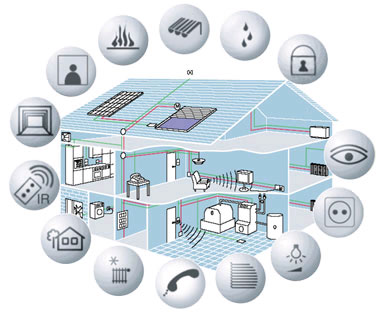
\includegraphics[scale=0.5]{Images/jpg/domotic.jpg}
    \\[2cm]

    % Author and supervisor
    \begin{minipage}{0.4\textwidth}
      \begin{flushleft} \large
        BAIZ Mamoune \\ MUNIER Marc \\
        Promo 2016\\
      \end{flushleft}
    \end{minipage}
    \begin{minipage}{0.4\textwidth}
      \begin{flushright} \large
        \emph{Encadrant :} M. Briffaut\\
      \end{flushright}
    \end{minipage}

    \vfill

    % Bottom of the page
    {\large 9 Février 2016}

  \end{center}
  \end{sffamily}
\end{titlepage}
}
%%%%%%%%%%%%%%%%%%%%%%%Page Vierge%%%%%%%%%%%%%%%%%%%%
\newpage
\newpage



%%%%%%%%%%%%%%%%%%%%% Remerciment %%%%%%%%%%%%%%%%%%%%
\newpage
\section*{Remerciement}
Au terme de notre formation à L’INSA Centre Val de Loire, et tout au long de ce projet il est nécessaire de remercier tous mes professeurs, ainsi que tout le corps professoral et administratif de notre établissement, auxquels nous tenons à rendre hommage pour leurs efforts prodigieux qu’ils n’ont cessé de fournir afin que nous puissions, mes collèges et moi, avoir une formation solide et rigoureuse ; pour leur encadrement tout au long de cette année, et pour leur disponibilité permanente. Nous n’oublierons pas de remercier spécialement M.Briffaut pour son soutien tout au long du projet, ainsi que ces précieux cours de "domotique" qui nous ont aidés à réaliser ce projet.\newline

%La vieillesse renouvelle la terreur à
%l’infini. Elle ramène l’être sans finir au
%commencement. Le commencement qu’au bord
%de la tombe j’entrevois est le \emph{porc}
%qu’en moi la mort ni l’insulte ne peuvent
%tuer. La terreur au bord de la tombe est
%divine et je m’enfonce dans la terreur dont
%je suis l’enfant.


%marc: ok pour moi peut etre revoir la forme
\clearpage
\newpage
%%%%%%%%%%%%%%%%%%%%%Résumé%%%%%%%%%%%%%%%%%%%%%%%%%%%
%\section*{Résumé}
%\vspace{40pt} 
%\label{chap-savoir}
%\begin{epigraphe}{Les proverbes Pr \textbf{21} 11}
%Quand on châtie le railleur, le simple s’assagit ;\\
%quand on instruit le sage, celui-ci gagne en savoir.
%\end{epigraphe}

 %  Votre résumé commence ici...
%   ...

%\newpage
%%%%%%%%%%%%%%%%%%%%%table des matières%%%%%%%%%%%%%%%
\tableofcontents
\clearpage

%%%%%%%%%%%PLAN
%
%\section*{Introduction} %(comment on a fait ce projet, en quoi il consiste, les enjeux)
%Mamoune
%Mamoune: Dans cette partie il est conseillé de prendre une photo représentant la conception 
%		C)	l'application
% 
%III)	Comment le mettre en place Marc
%V)		Nos difficulté
%VII)	Conclusion
%
%V)		Nos diffficultés difficulté
%VII)	Conclusion (fini)
%
%Ne pas oublier l'annexe
%Ne pas oublier le glossaire.
%
% chaque partie est à ecrire dans un fichier indépandant du main
% il suffit de rajouter la ligne suivante pour inclure ces écrits
%\input ./maPartie.tex %sans saut de ligne
%
%%%%%%%%%%%%%%%%%%%


%%%%%%%%%%%%%%%%%%%%%%%%%%%%%%%%%%%%%%%%%%%%%%%%%%%%%%

\newpage
\chapter{Introduction}

Ce projet se présente comme une très bonne expérience sur le plan théorique et pratique, car il permet de concevoir une première approche sur le monde des objets connectés et plus spécialement en domotique. Il constitue aussi une occasion unique pour mettre en évidence le cumul des connaissances que nous avons acquis tout au long de notre formation spécialisée en sécurité ubiquitaire.


De ce fait, notre binôme a décidé de réaliser un projet concernant la domotique. Toutefois, il est nécessaire de définir ce qu'est la domotique. La domotique est l'ensemble des techniques de l'électronique, de physique du bâtiment, d'automatisme, de l'informatique et des télécommunications utilisées dans les bâtiments, plus ou moins « interopérables » et permettant de centraliser le contrôle des différents systèmes et sous-systèmes de la maison et de l'entreprise (chauffage, volets roulants, porte de garage, 
portail d'entrée, prises électriques, etc.). La domotique vise à apporter des solutions techniques pour répondre aux besoins de 
confort (gestion d'énergie, optimisation de l'éclairage et du chauffage), de sécurité (alarme) et de communication (commandes à 
distance, signaux visuels ou sonores, etc.) que l'on peut retrouver dans les maisons, les hôtels, les lieux publics, etc.


Ce projet consiste alors à créer une petite centrale domotique grâce à une raspberry, permettant d'informer l'utilisateur sur certaines données reçues par des capteurs. Cette mini centrale permettera alors à l'utilisateur d'améliorer son confort et surtout sa sécurité. Ceci ne pourrait être que bénéfique envers les utilisateurs potentiels. La domotique est de plus en plus présente dans notre quotidien. Grâce à elle nous pouvons alors économiser de l'énergie (gestion du chauffage, gestion de l'éclairage, gestion des volets), augmenter l'autonomie des personnes à mobilité reduite (assistance à l'ouverture des portes, des fenêtres, des volets, pilotage des appareils électriques, commande vocale) ou encore améliorer la sécurité de nos habitations (système d'alarme). La mise en place d'un système domotisé peut se faire dès la construction d'un bâtiment (norme KNX), lors d'une rénovation, ou encore de façon ponctuelle (norme X10).




%%%%%%%%%%%%%%%%%%%%%%%%part II %%%%%%%%%%%%%%%%%%%%%%

\newpage
\chapter{Presentation du projet}
\section{Les outils} 
Afin de réaliser ce projet, quelques outils et éléments nous ont été indispensables. Tout d'abord, la centrale qui contrôle tout le système de domotique: La Raspberry Pi.

Le Raspberry Pi est un nano-ordinateur monocarte à processeur ARM conçu par le créateur de jeux vidéo David Braben, dans le cadre de sa fondation Raspberry Pi. Cet ordinateur, qui a la taille d'une carte de crédit, est destiné à encourager l'apprentissage de la programmation informatique. Il permet l'exécution de plusieurs variantes du système d'exploitation libre GNU/Linux et des logiciels compatibles à plusieurs protocoles de domotique. Il est fourni nu (carte mère seule, sans boîtier, alimentation, clavier, souris ni écran) dans l'objectif de diminuer les coûts et de permettre l'utilisation de matériel de récupération.
Cet outil est alors la pièce maîtresse de notre projet domotique. 
\subsection{Description de la raspberry pi 2}
%TODO
%\begin{itemize}
%\item[LA FIBARO Wall Plug] \hfill \\
\begin{figure}[h]
	\center
	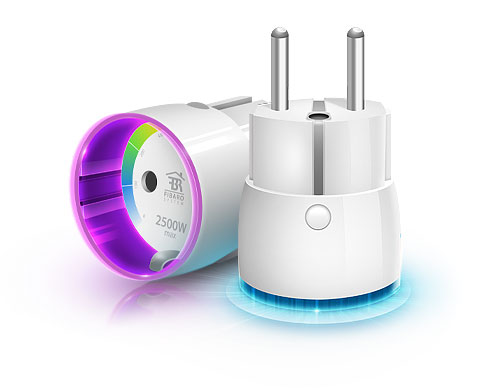
\includegraphics[scale=0.5]{./Images/jpg/WallPlug_FibaroDevice.jpg}
	\caption{Capteur d'énergie}
\end{figure}
\begin{description}
	\item[Environnement] \hfill \\ Linux (Debian, Fedora et ArchLinux), RISC OS , Windows IOT
	\item[Système d'exploitation] \hfill \\ Linux (Raspbian, Pidora, et Arch Linux ARM gentoo), RISC OS, FreeBSD, NetBSD, Windows 10 IoT (uniquement compatible avec le Raspberry Pi 2), Plan 9
	\item[Alimentation] \hfill \\ Micro-USB 5 V
	\item[Processeur] \hfill \\
		\begin{itemize}
			\item Broadcom BCM2835 - ARM1176JZF-S 700 MHz (modèle 1) ou 1 GHz (Modèle Zero)1
			\item Broadcom BCM2836 - Cortex-A7 900 MHz (modèle 2)
		\end{itemize}

	\item[Stockage] \hfill \\ Carte SD (A, B), Carte microSD (A+,B+,2)
	\item[Mémoire] 
		\begin{itemize}
			\item 256 Mo (modèle A et A+)
			\item 256 Mo (modèle B rev 1)
			\item 512 Mo (modèle B rev 2 et B+)
			\item 1 Go (modèle 2)
		\end{itemize}

	\item[Carte graphique] \hfill \\ Broadcom VideoCore IV1,
	\item[Connectivité] \hfill \\ USB, Ethernet (modèle B, B+ ,2) (RJ45), HDMI, RCA, Jack 3,5 mm, Micro USB
	\item[Dimensions] \hfill \\ 
		\begin{itemize}
			\item 85,60 mm × 53,98 mm × 17 mm (A, B, B+),
			\item 65 mm × 53,98 mm × 17 mm (A+),
			\item 65 mm × 30 mm × 5 mm (Zero)
		\end{itemize}
	\item[Poids] \hfill \\ 44,885 g (A, B, B+), 23 g (A+)
\end{description}

\subsection{Les composants utilisés}
Afin de savoir les données concernant le milieu ambiant contournant la centrale de domotique (la raspberry pi2), il est nécessaire d'utiliser des capteurs pour capturer les données que nous souhaitons, mais aussi d'une antenne posée sur la raspberry analysant les données qu'elle reçoit depuis les capteurs.

\subsubsection{Antenne}
Nous avons utilisé une antenne Z-Wave. Z-Wave est un protocole radio conçu pour la domotique, facilement intégré avec la raspberry pi2. Z-Wave fonctionne dans la gamme de fréquence sous-gigahertz, qui dépend des régions (868 MHz en Europe, 908 MHz aux US, et d'autres fréquences suivant les bandes ISM des régions). La portée est d'environ 50 m (davantage en extérieur, moins en intérieur). La technologie utilise la technologie du maillage (mesh) pour augmenter la portée et la fiabilité.

\begin{figure}[h]
	\center
	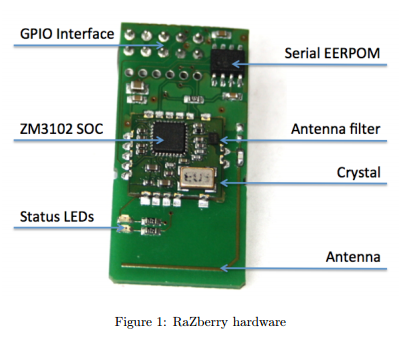
\includegraphics[scale=0.5]{./Images/png/Zwave.png}\newline
	\caption{Antenne Zwave}
\end{figure}

Etant donné que le protocole Z-Wave se base sur une seule plage de fréquence il est donc vulnérable à un brouilleur de fréquence.
 De plus le protocole lui-même semble souffrir de problèmes de sécurité. Dans l'état actuel de cette norme, il semble plus prudent de ne confier à Z-Wave que des tâches domotiques limitées aux éléments dont le dysfonctionnement ou le piratage ne pose pas de problème.
\subsubsection{Les Capteurs}

\begin{description}
\item[FIBARO Smoke Sensor] \hfill \\

\begin{figure}[h]
	\center
	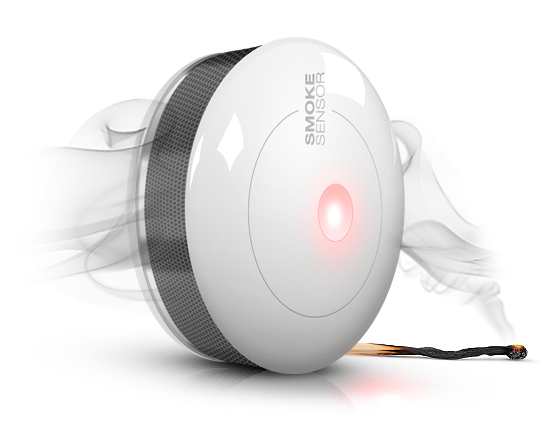
\includegraphics[scale=0.4]{./Images/png/smoke.png}
	\caption{Capteur de fumeé}
\end{figure}

Ce détecteur est très sensible à la fumée, mais pas juste à la fumée. Certains matériaux brûlent avant de capter la fumée sous haute température.
Voilà pourquoi les ingénieurs de  FIBARO ont décidé d'inclure une protection supplémentaire: un capteur de fumée sous la forme d'un capteur de température.
 Si la quantité de fumée n'est pas assez suffisante pour déclencher l'alarme, l'appareil sera toujours en mesure de détecter la menace.
En effet, il est sensible à un changement rapide de température provoqué par un feu. Il détecte aussi lorsque la température dépasse les 54°C. Ceci est alors suffisant pour le capteur de fumée pour découvrir la menace et signaler les utilisateurs à ce sujet. 

\item[FIBARO Flood Sensor] \hfill \\

\begin{figure}[h!]
	\center
	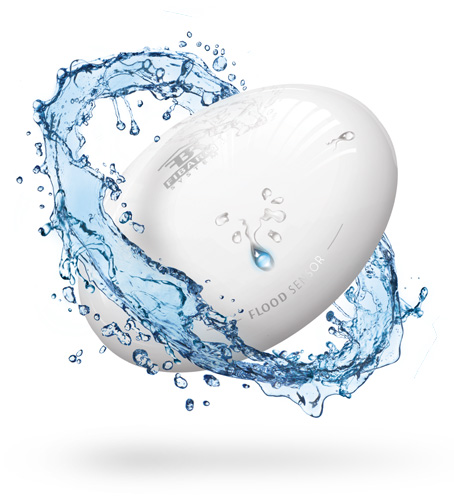
\includegraphics[scale=0.5]{./Images/jpg/floodSensor_FibaroDevice.jpg}
	\caption{Capteur d'innondation}
\end{figure}

Le capteur d'innondation FIBARO, une taille compacte et une grande variété de fonctions supplémentaires .Ce capteur est tout simplement remarquable !Ce dispositif unique peut vous garantir une sécurité optimale. Avec sa technologie de pointe et de précision, le capteur d'innondation Fibaro vous alerte de crue menaçante, ou un changement radical de température. Tout en étant sans entretien et sans la nécessité d'une installation professionnelle.



\item[LA FIBARO Wall Plug] \hfill \\
\begin{figure}[h!]
	\center
	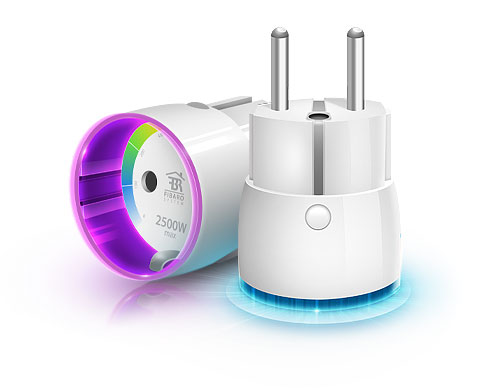
\includegraphics[scale=0.5]{./Images/jpg/WallPlug_FibaroDevice.jpg}
	\caption{Capteur d'énergie}
\end{figure}
Ce capteur a la forme une prise murale. Elle peut indiquer, la consommation de la puissance électrique qui passe en courant, en temps réel sous forme d'un halo lumineux autour de la prise.

Ce capteur respecte des normes de sécurité très exigeantes, et obligatoires dans certains pays nordiques.

Il permet en outre de connaître la consomonation en temps réel mais aussi la consomation moyenne. Ce capteur donne aussi la possibilité d'éteindre et d'allumer la prise à distance.

\end{description}



\subsection{Le logiciel Domoticz}
Domoticz est un logiciel libre de gestion de domotique qui a pour but d’être exécutable sur un grand nombre de machines différente. Et ce qui fait son principal atout, c’est que le Raspberry Pi fait partie des machines sur lesquelles il peut tourner ! Ce qui permet donc d’en faire une machine dédiée aux opérations domotiques à prix très réduit. 
Neamoins, ce logiciel présente quelques difficultés au niveau de l'incorporation des capteurs. Suite à ce de problème nous avons choisi d'utiliser un autre logiciel.

\subsection{Le logiciel ZwaveMe}
Nous avons aussi utilisé, l'interface web proposée par Z-WaveMe.
Cette inteface permet d'ajouter trés simplement des capteurs et sa configration est simple.
Ce logiciel propose une inerface web disponible sur le port 8083. Grâce à ce site internet, l'utilisateur peut ajouter et supprimer des capteurs, modifier leurs configurations et leurs options.
Enfin, nous pouvons installer d'autres aplications disponibles sur internet. 
Donnons à titre d'exemple l'application IfThen. Elle permet de générer des scénarios en respectant des conditions (If ---> Then). Avec cet outil, nous avons pu générer plusieurs scénarios. Des vidéos de démonstration se trouvent dans ces liens.\newline
\url{https://www.youtube.com/watch?v=nNWe8rKhf1o&feature=youtu.be}
Le scénario mis en place dans ces vidéo, simule une innodation. Suite à l'alarme du capteur flood\_Sensor, ZWaveMe désactive les prises éléctriques. 

Un autre point fort du logiciel ZwaveMe est la présence d'un fichier de log permetant à l'utilisateur de pouvoir visualiser tout ce qui se passe pendant la journée concernant les capteurs.

\subsection{L'application Android}
Afin d'améliorer notre projet, nous avons décidé de réaliser une application android, permettant aux clients distants de pouvoir se connecter à distance pour accéder aux données partagées par la centrale domotique. Ainsi il pourra gérer son domicile, et créer des scénarios après certaines conditions. Sur la page d'accueil de l'application, l'utilisateur devra choisir une habitation qu'il posséde afin qu'il puisse découvrir l'état de ce dernier. Il a aussi la possibilité d'en rajouter une.\newline
Cette application utilise une fonctionalité de ZwaveMe. En effet, ZWaveMe permet de pouvoir contrôler un capteur, connaitre son etat et le configurer grâce à des requettes http. 
La réponse de ces requêtes est en Json. 


Néanmoins, faute de temps, nous n'avons pas pu aboutir au résultat souhaité, l'application affiche une page générique par défaut pour toutes les habitations. Cette application n'était pas un élément crucial de notre projet, mais elle aurait pu l'améliorer considérablement. Cette thématique pourra alors ouvrir la possibilité de générer de nouveaux projets, essayant de répondre à ce besoin.\newline
Le code source de cette application sera mis en annexe.\newline


%%%%%%%%%%%%%%%%%%%%%%%%partie III%%%%%%%%%%%%%%%%%%%%

\input ./III_MiseEnPlace.tex %sans saut de ligne

%%%%%%%%%%%%%%%%%%%%%%%%%%%%%%%%%%%%%%%%%%%%%%%%%%%%%%%
\newpage
\chapter{Les problèmes rencontrés}
Tout au long du projet, nous avons rencontré quelques difficultés, que nous avons réussi à résoudre. Dans ce chapitre, nous allons décrire tous les problèmes rencontrés, et les solutions que nous avons mises en oeuve pour résoudre ces derniers.
\subsection{Cartes SD grillées }
Avant de commencer le projet, il nous a été donné deux raspberry Pi et tous les composants qui vont nous permettre de connecter la raspberry Pi2 et de s'en servir.\newline
Parmi ces éléments, des cartes SD nous ont été offertes pour réaliser le projet. Néanmoins, parmi plusieurs cartes SD, un grand nombre d'entre elles était non fonctionnellles, et d'autres ont cessé de fonctionner après un certain nombre d'essai avec la raspberry Pi2.\newline
A cause des nombreuses installations de système que nous avons dû réaliser tout au long du projet, nous avons décidé de travailler avec une seule raspberry Pi, et de changer la version de la raspberry Pi en raspberry Pi2, pour des raisons d'optimisation. Après cette manoeuvre, nous avons pu avancer plus rapidement, sans aucun souci de connexion ni de mémoire.
\subsection{Antenne Z-Wave}
Afin d'analyser les données des capteurs, une Antenne Z-Wave nous a été donnée. Cependant, parmi deux des antennes Z-Wave données une ne marchait pas, ceci nous a encore poussé à éliminer une raspberry et de réaliser le projet avec une seule raspberry.
\subsection{Arrivée tardive du matériel (Antenne Z-Wave+Capteurs)}
Afin de réaliser le projet, du matériel spécifique nous était nécéssaire, M.Briffaut nous a commandé ce matériel.
Toutefois, le matériel est arrivé un peu tardivement. Durant ce temps, nous nous sommes bien documentés dans le but de mieux connaitre la domotique et ses enjeux. Nous avons profité de ce temps pour installer le système adéquate sur nos raspberry respectives.   

\newpage
\chapter{Conclusion}
De nos jours, le marché de la domotique est devenu un des projets les plus prometteurs, surtout avec la démocratisation des tablettes et smartphones, la fiabilité des technologies sans fil et l'émergence des objets connectés. Toutes ces conditions affirment que la maison intelligente est un véritable marché de masse. Le nouveau paysage technologique permet en effet de proposer des solutions domotiques moins chères, plus évolutives et intuitives et surtout adaptées aux besoins des consommateurs (confort au sein du logement, économie d'énergie, sécurisation des biens, autonomie des personnes dépendantes, etc.).\newline

Durant le présent projet, il nous a été confié comme mission de réaliser une centrale domotique, réalisant des tâches visant à sécuriser la vie des utilisateurs et d'améliorer leur confort. Nous étions alors dans l'obligation de mieux connaitre le monde de la domotique, afin que nous puissions mieux gérer le projet.
Après avoir approfondi nos connaissances, nous avons alors réussi à réaliser un projet en domotique permettant de gérer quelques capteurs et de créer des scénarios à l'issue de situations spécifiques.\newline

L'élaboration de ce travail nous a permis d'une part, d'approfondir nos connaissances acquises et le savoir faire que nous avons pu réaliser tout au long de cette année de spécialité 2SU, et d'autre part de découvrir les solutions que proposent le monde de la domotique.\newline

%%%%%%%%%%%  ANNEXE %%%%%%%%%%%%%%%%%%%
%%%%%%%%%%%%%Index des images%%%%%%%%%%
\newpage
\chapter{ANNEXES}
\newpage
\section{Index des images}
\listoffigures
%%%%%%%%%%%%%%%%%%%%%%%%%%%%%%%%%%%%%%%
\newpage

\section{Caractéristique des capteurs utilisés}
\subsection{Caractéristiques du capteur de fumée FIBARO}

\begin{itemize}

\item Ce capteur répond à la nouvelle norme EN14604


\item Fonction "boite noire" (mémoire des événements).


\item Sans-fil Z-Wave+.


\item Design et matériaux nobles.


\item Compact avec seulement 6,5x2,8cm


\item Sensibilité réglable.


\item Bouton de configuration et d'indication multicolore.


\item Alimentation par pile fournie 


\item Autonomie de 3 ans env. (peut varier suivant les paramètres de réveil et de transmission des températures).


\item Garantie 2 ans


\item Sans-fil Z-Wave+.
\end{itemize}
\subsection{Caractéristique Wall plug}

\begin{itemize}

\item Protection enfants et fonction veilleuse.


\item Configuration ultra-simple grâce à l'unique bouton est aux indications lumineuses.


\item La puissance maximale autorisée est de *2500W (11A) avec charge résistive (éclairage incandescent / halogène, radiateur, four à convection, etc.).
    

\item La puissance maximal autorisé est de *1500W (8A) avec charge capacitive (ampoules LED ou Fluo, TV et appareils électroniques, four MO, plaques à indiction,etc.). En cas de doute sur le type de charge, ne dépassez pas 1500W.


\item Fonction répéteur pour étendre le réseau Z-Wave.


\item Modèle avec prise Française (Type E)


\item Garantie 2 ans 

\end{itemize}
\section{Code de l'application Android}

Pour retrouver le code du programme Android réalisé, veuillez suivre le lien suivant:  \url{https://github.com/marcMunier/INSAdom/tree/master/InsaDomApp}


\section{ Ajout et configuration d'un capteur dans ZWaveMe}

La section suivante décrit les étapes pour configurer et ajouter un capteur avec l'interface Web de ZWaveMe


\subsection{Ajout d'un capteur sur l'interface ZwaveMe}

\begin{itemize}

\item Pour ajouter un élément, il faut tout d'abord appuyer sur la touche paramètre en haut à droite, et choisir Devices.

\begin{figure}[h]
	\center
	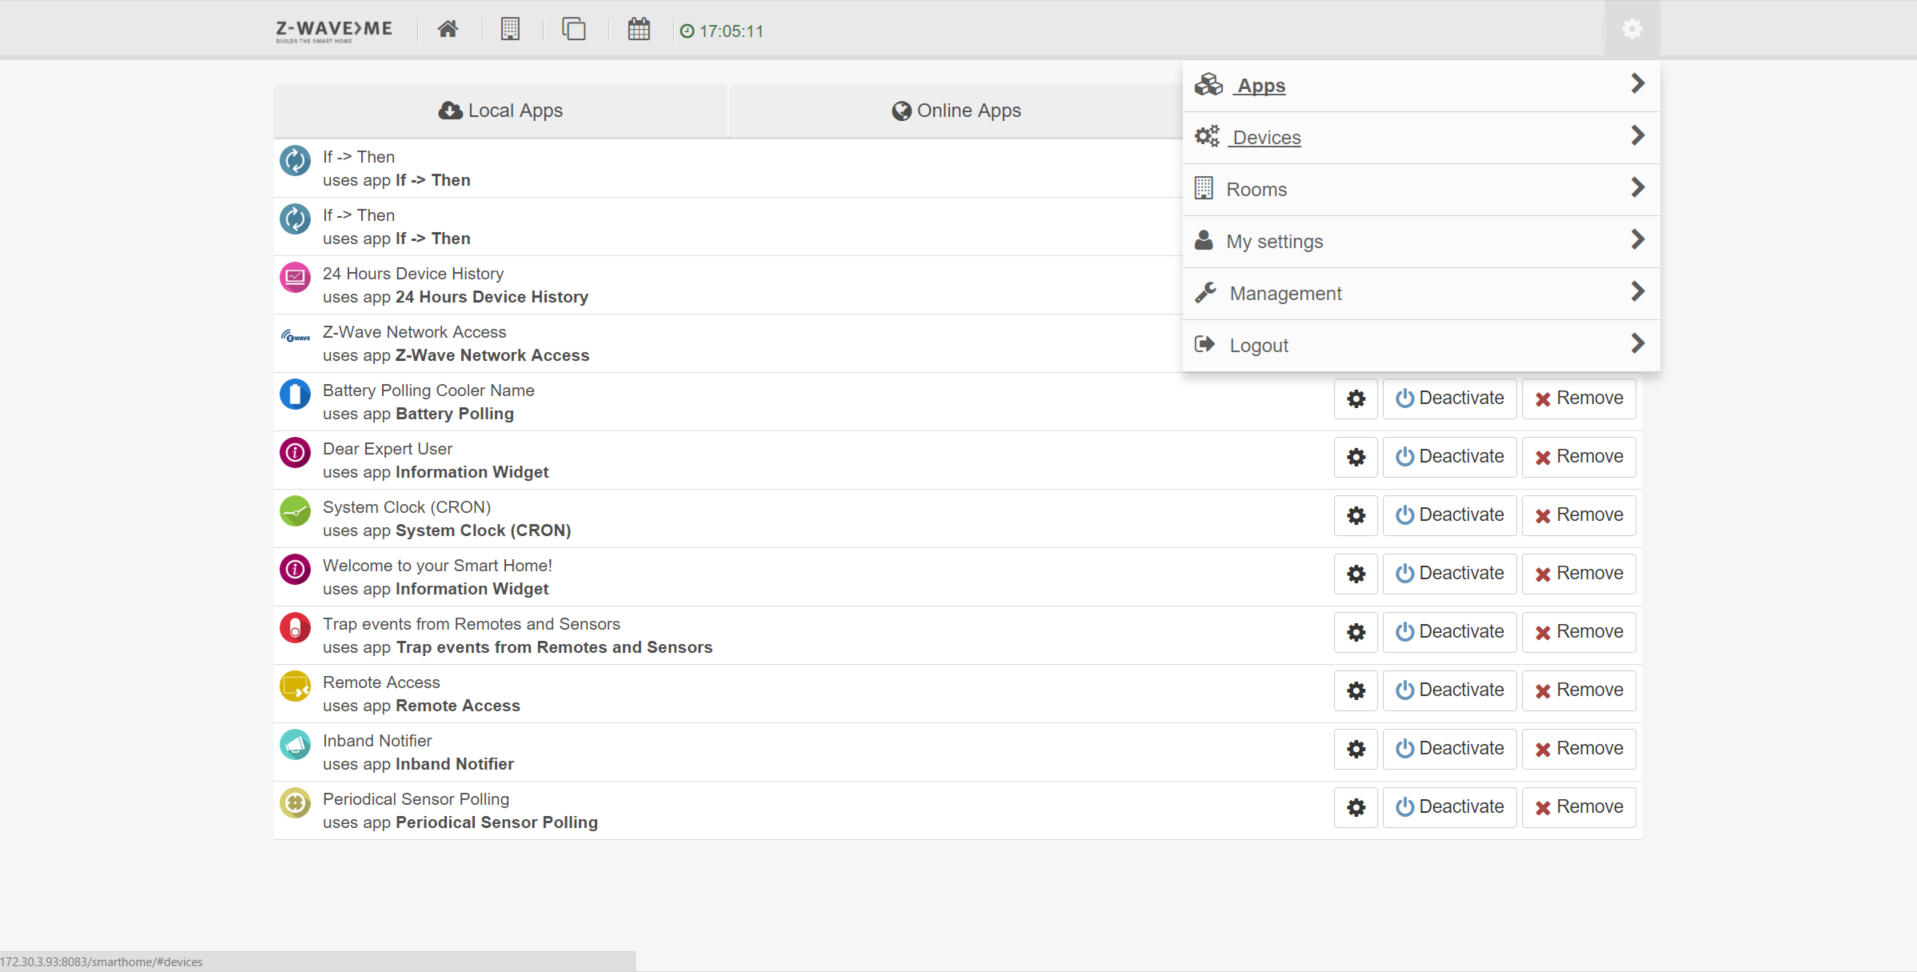
\includegraphics[scale=0.5]{./Images/png/menu_zwaveme.png}
	\caption{Menu de ZWaveMe}
\end{figure}


\item Appuyez dans la partie ZWave sur Add new.


\begin{figure}[h]
	\center
	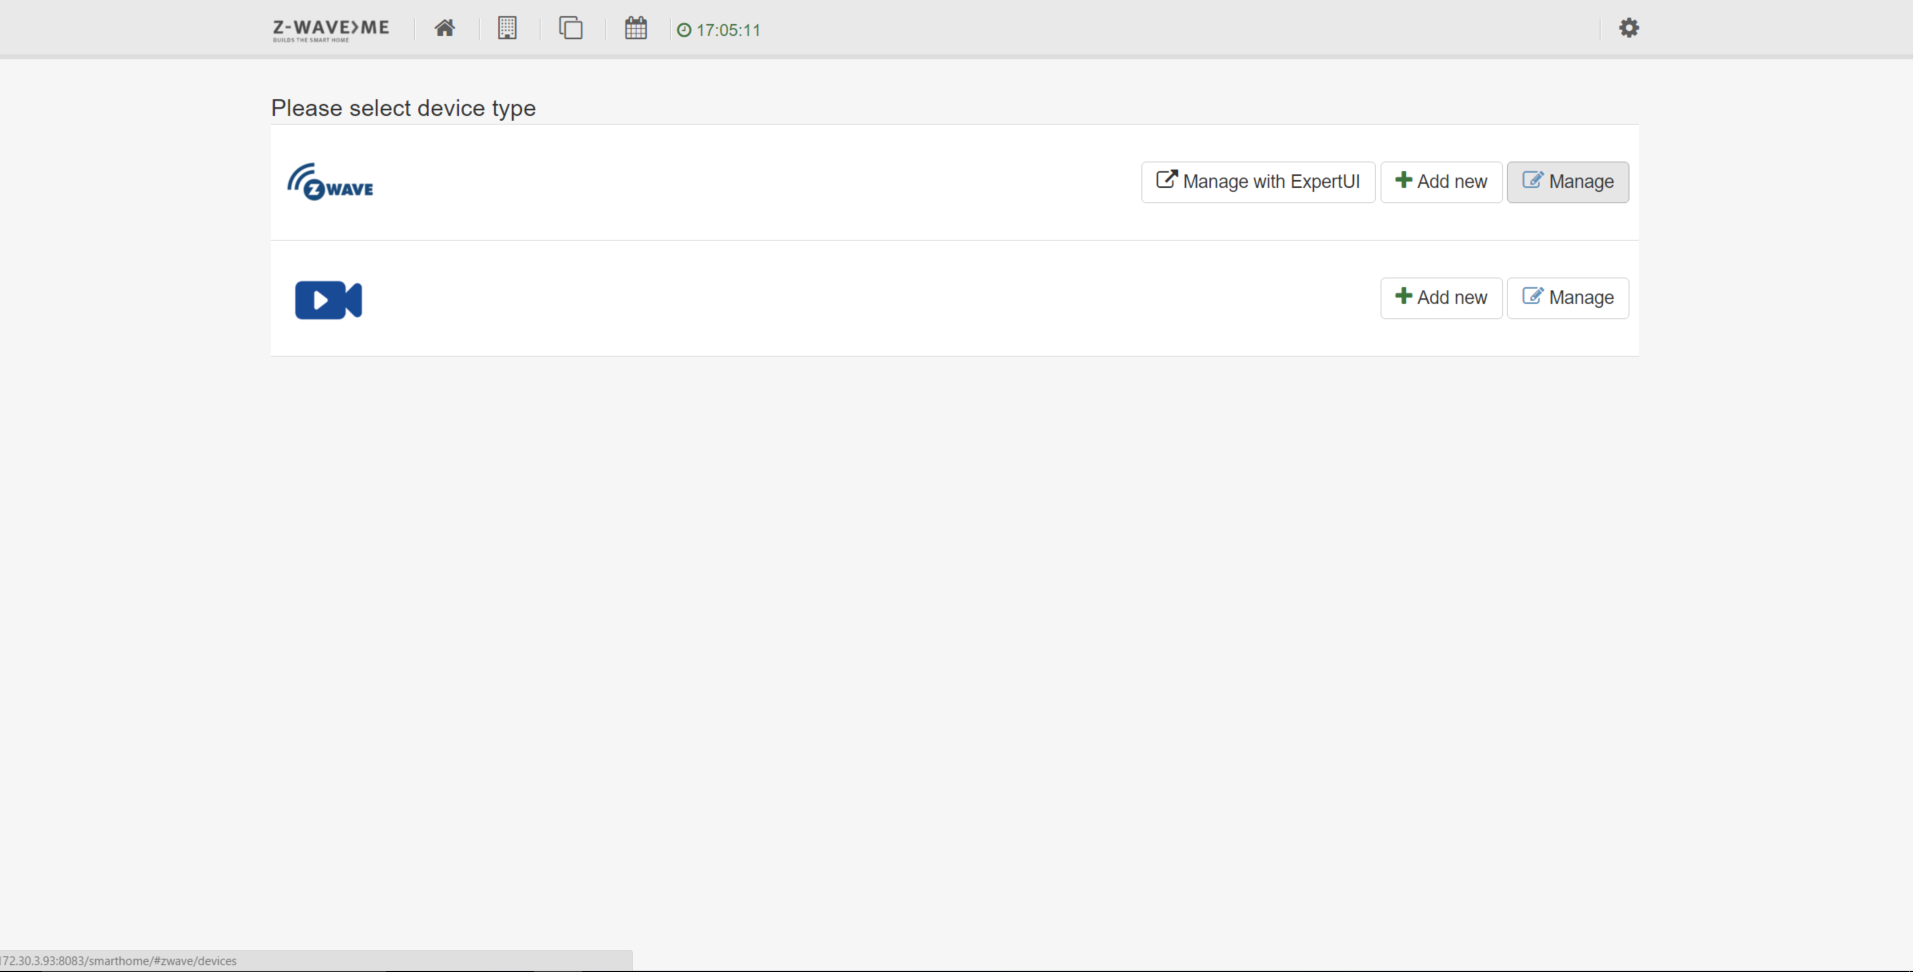
\includegraphics[scale=0.5]{./Images/png/devices_zwaveme.png}
	\caption{Menu des devices ZWaveMe}
\end{figure}


\item Appuyez sur "Start inclusion" et réveillez votre matériel en suivant les règles de chaque capteur

\begin{figure}[h]
	\center
	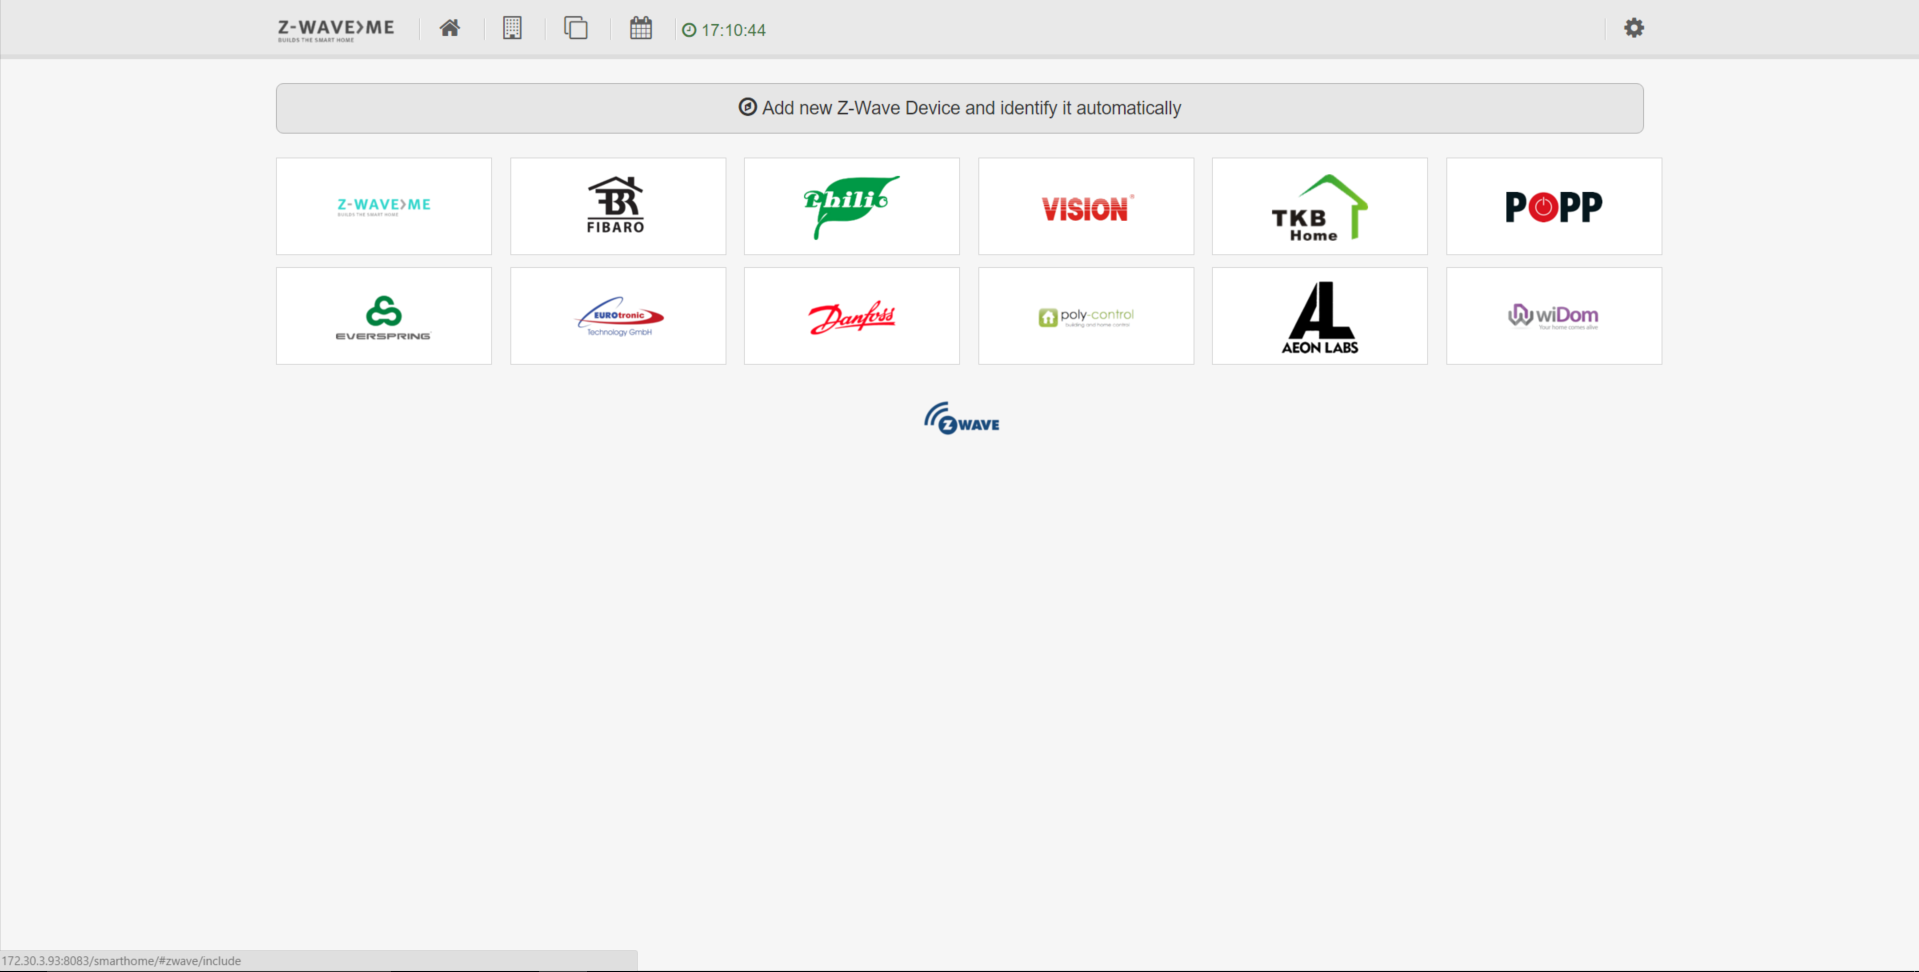
\includegraphics[scale=0.5]{./Images/png/add_zwaveme.png}
	\caption{Menu ajouter device}
\end{figure}

\item Attendre un instant

\begin{figure}[h]
	\center
	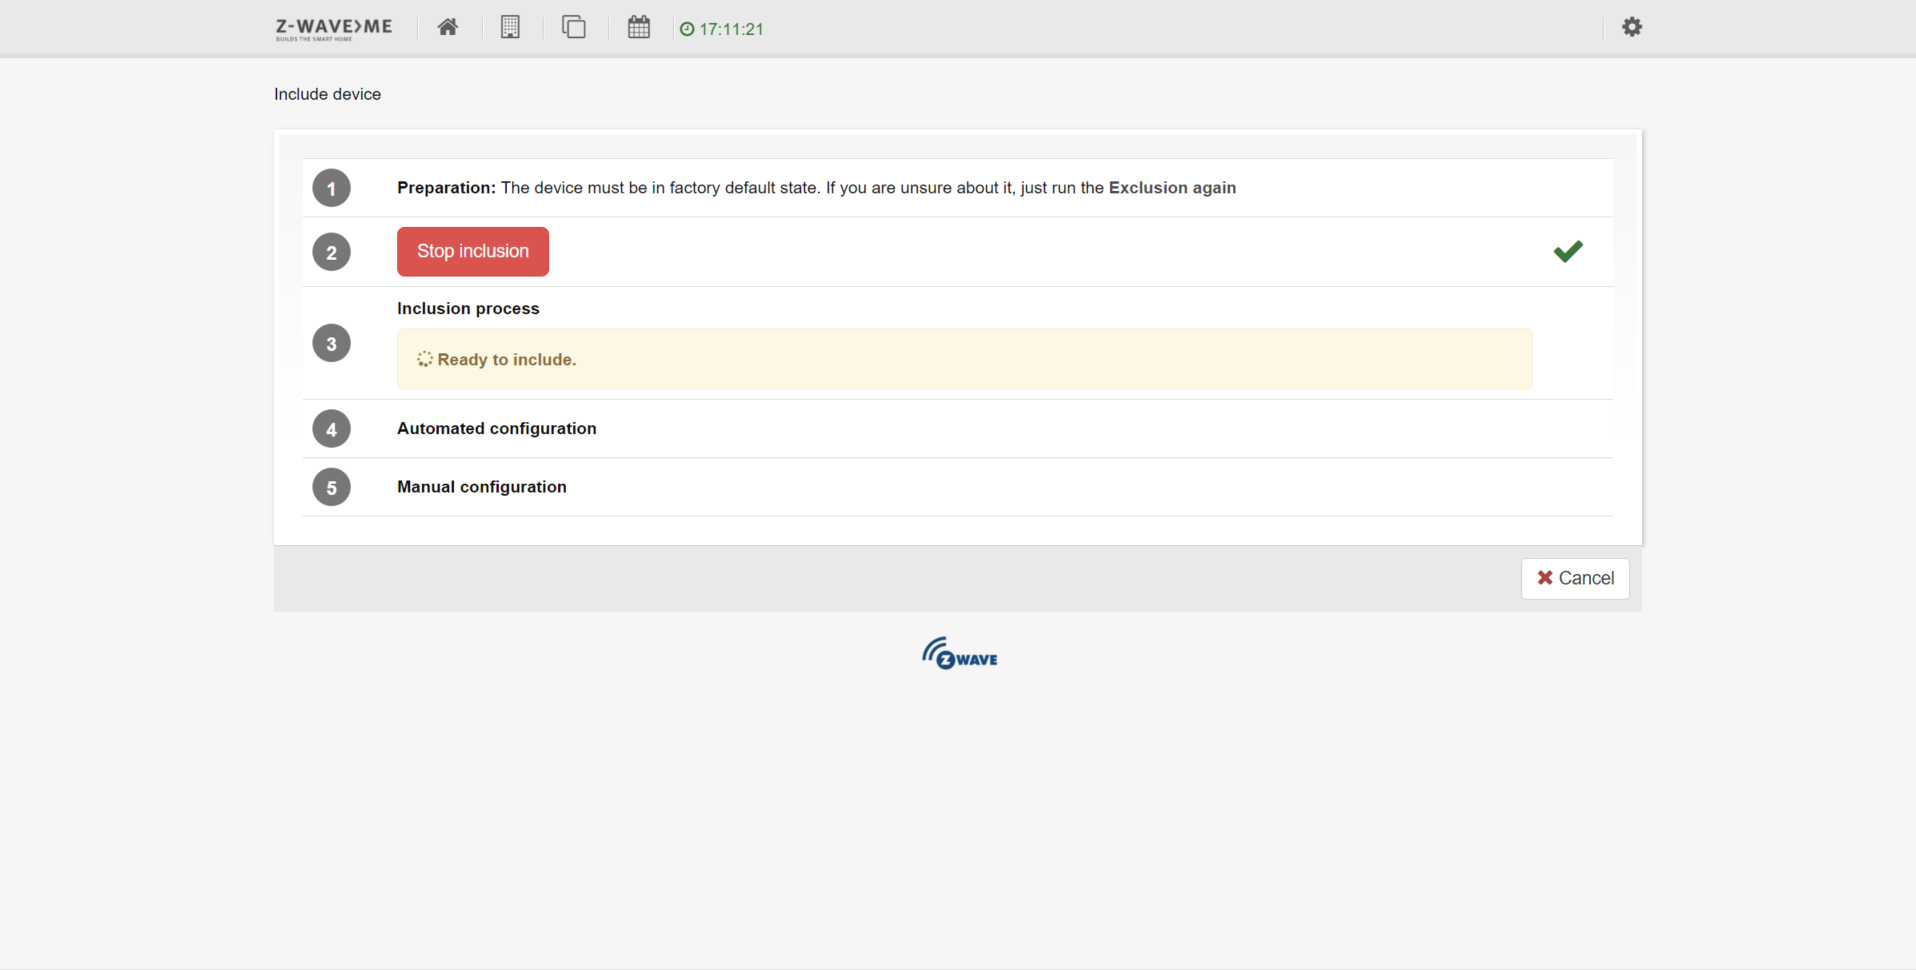
\includegraphics[scale=0.5]{./Images/png/add2_zwaveme.png}
	\caption{Menu ajouter device}
\end{figure}


\item L'élément est ajouté avec succès

\begin{figure}[h]
	\center
	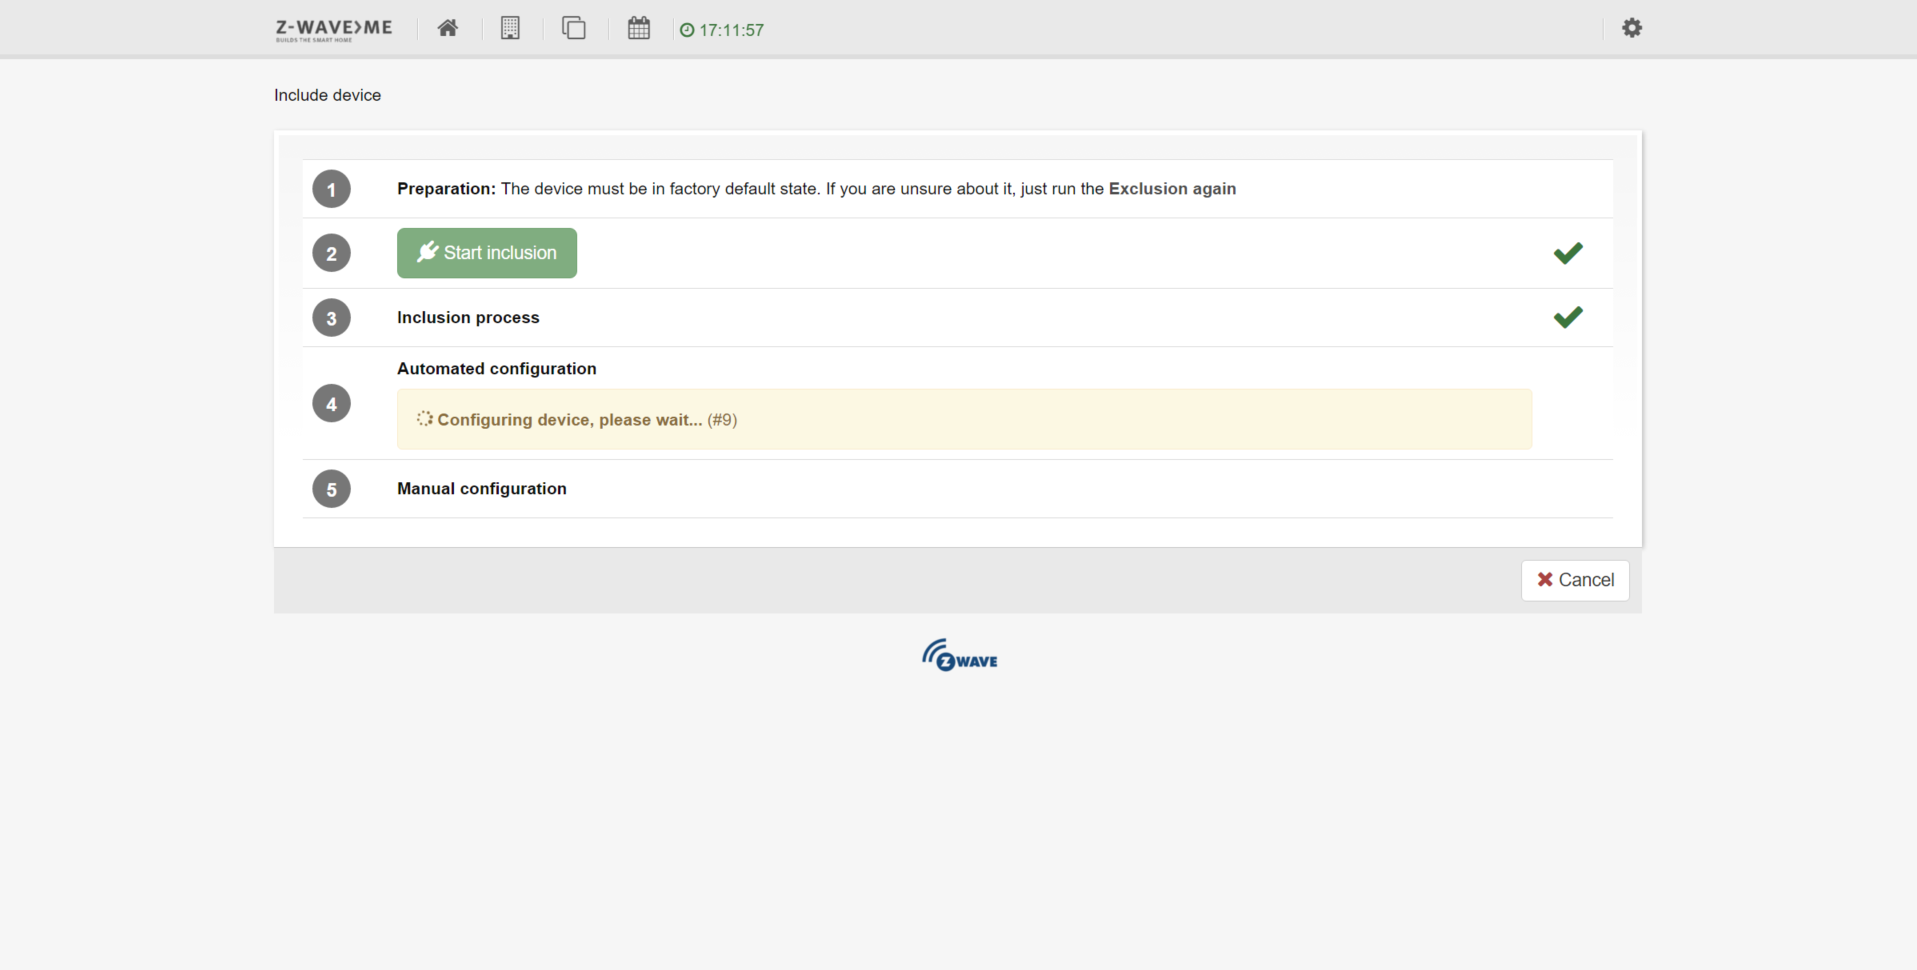
\includegraphics[scale=0.5]{./Images/png/add3_zwaveme.png}
	\caption{Menu ajouter device}
\end{figure}

\begin{figure}[h]
	\center
	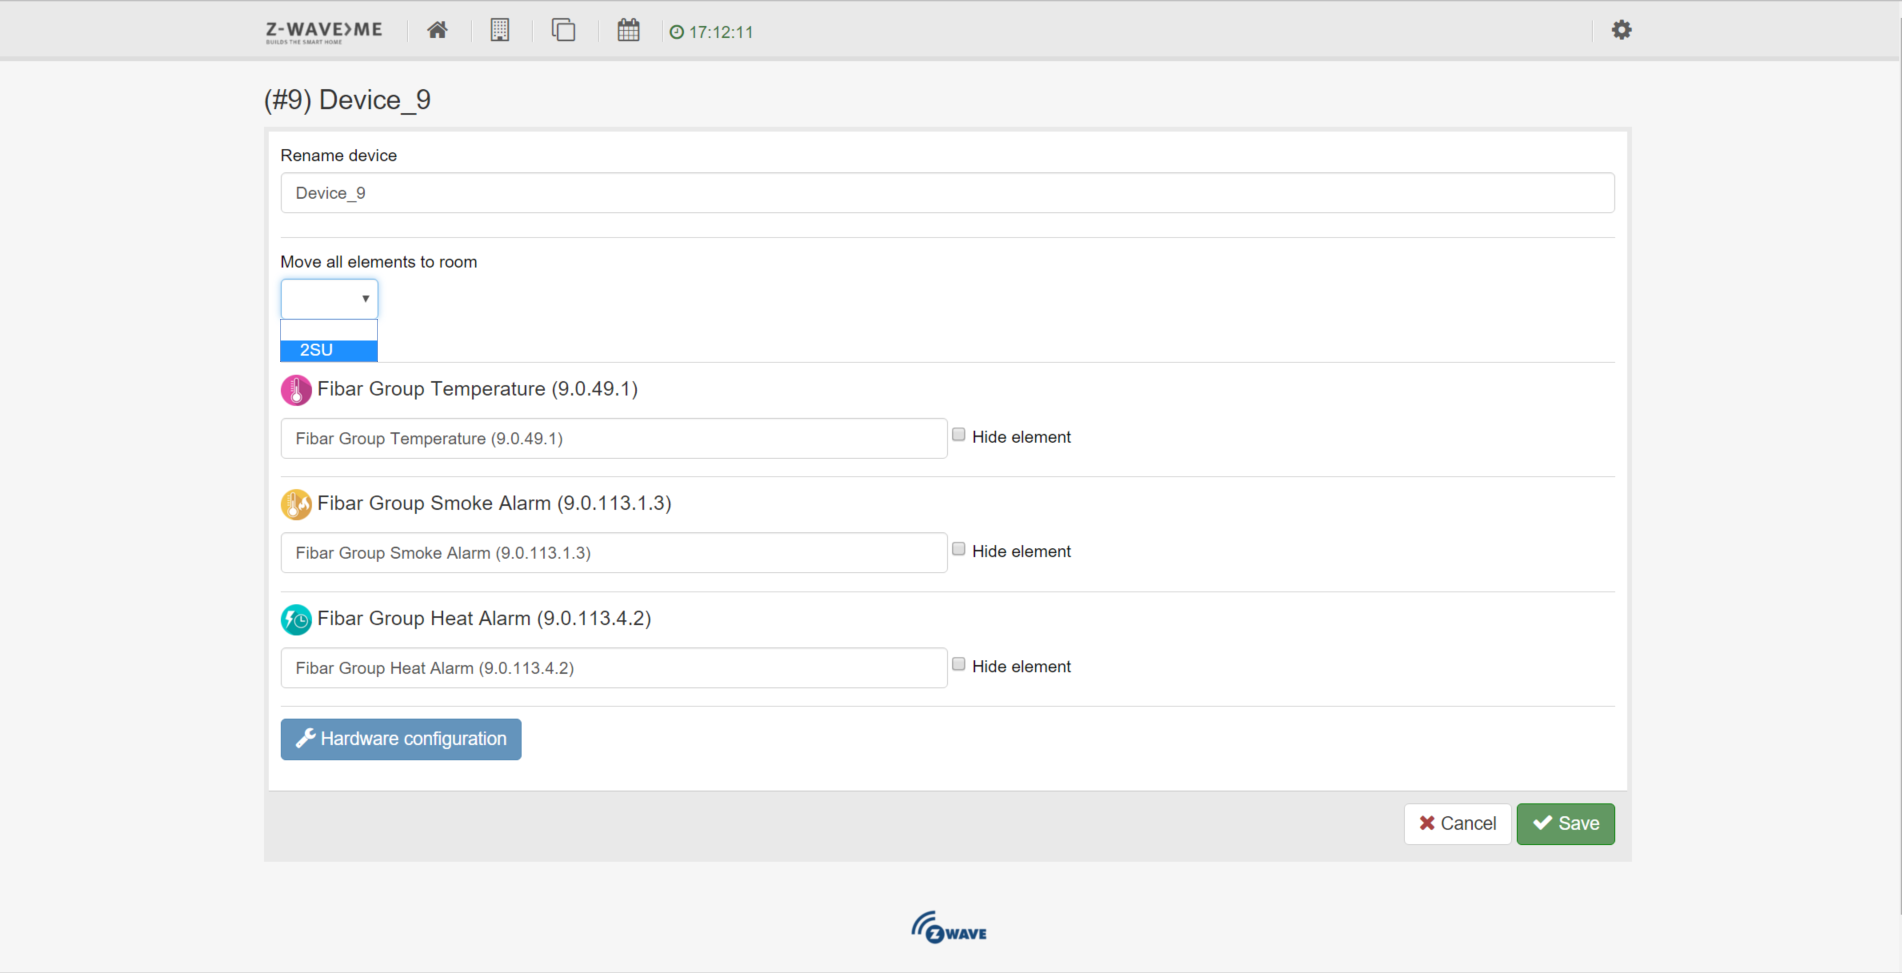
\includegraphics[scale=0.5]{./Images/png/add4_zwaveme.png}
	\caption{Menu ajouter device}
\end{figure}


\item Les capteurs disponibles

\begin{figure}[h]
	\center
	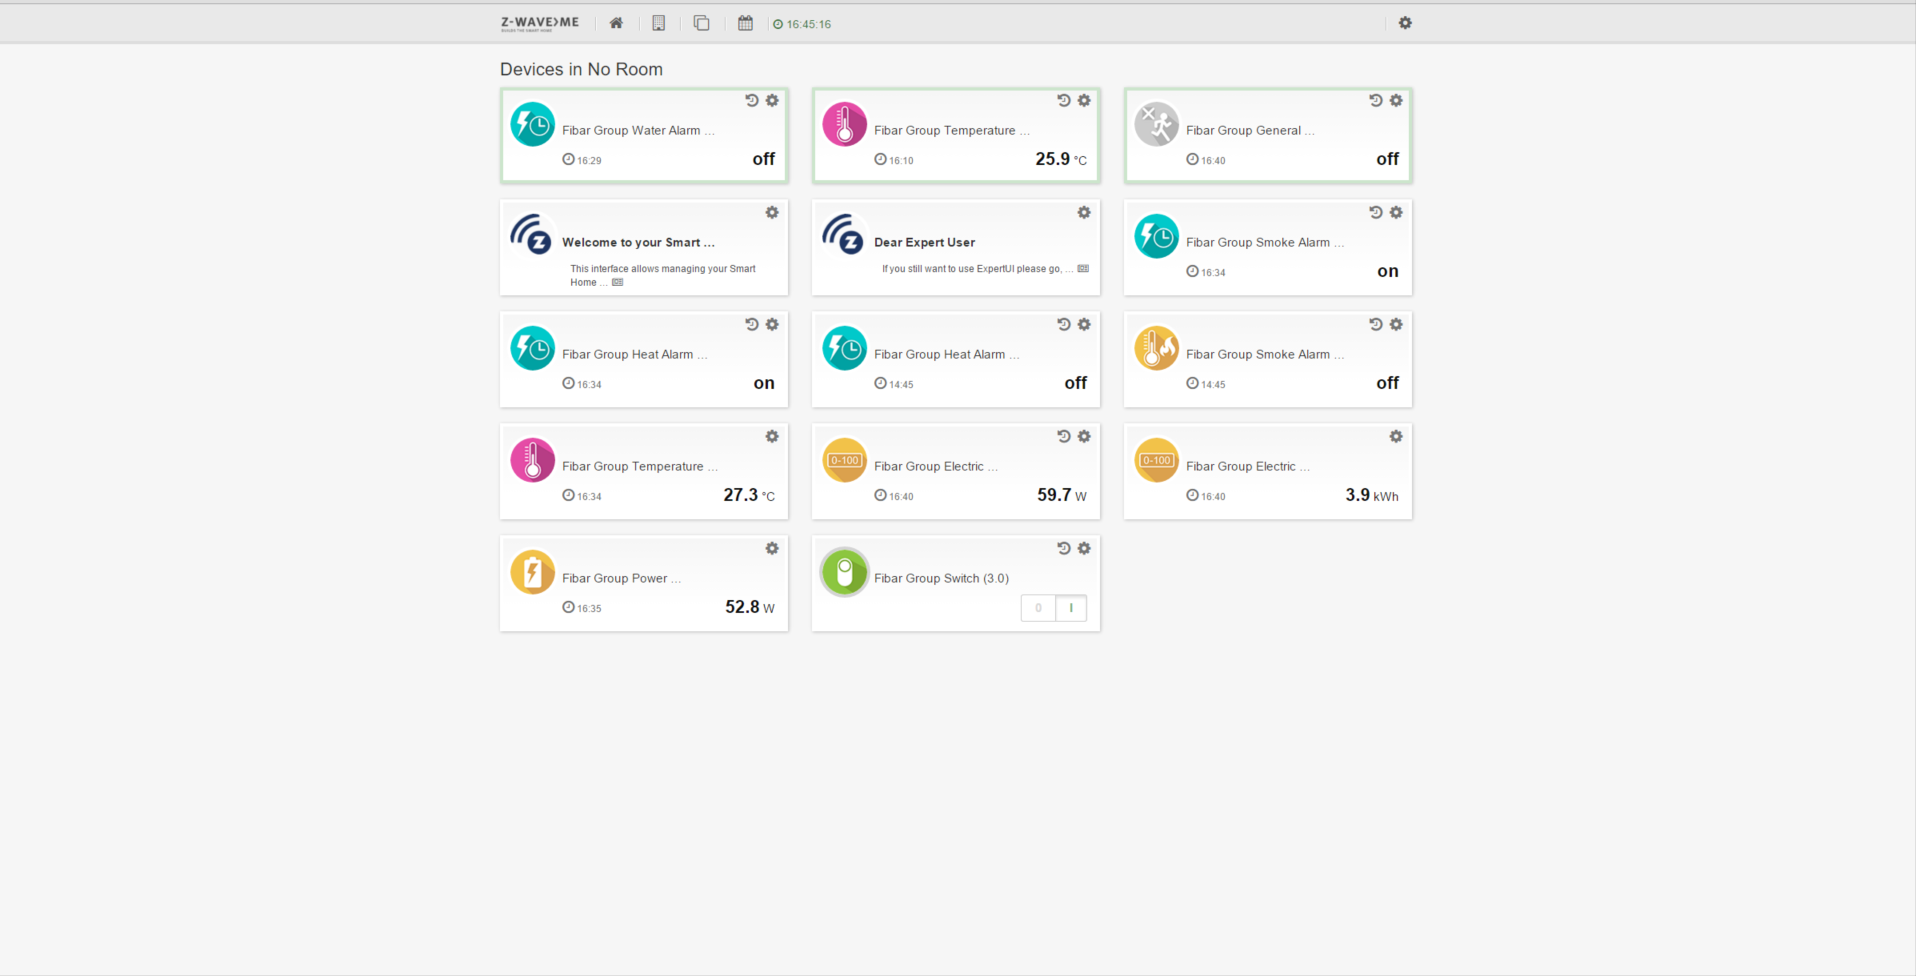
\includegraphics[scale=0.5]{./Images/png/ecranCapteur.png}
	\caption{Ecran ZWaveMe capteur}
\end{figure}



\begin{figure}[h]
	\center
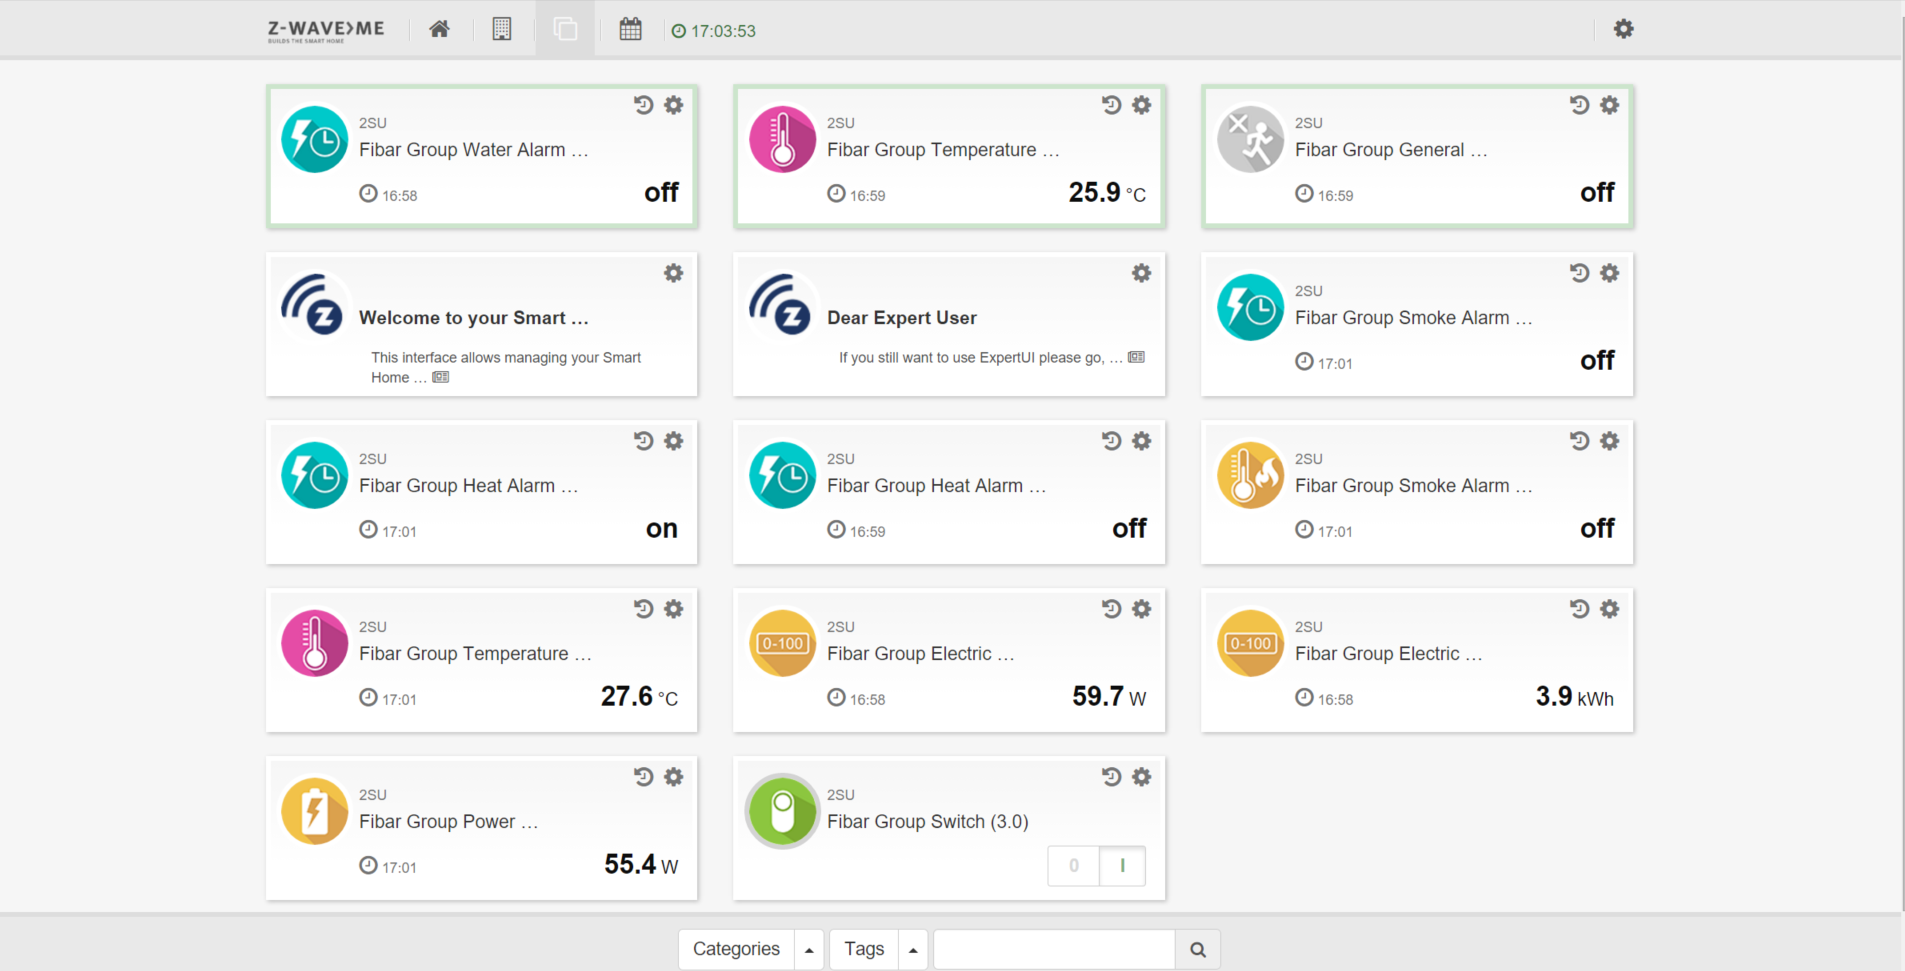
\includegraphics[scale=0.5]{./Images/png/device_zwaveme.png}
	\caption{ZwaveMe device}
\end{figure}


Il existe deux modes de gestion des capteurs avec l'interface ZWaveMe, le mode home et le mode expert:


\item Le mode home

\begin{figure}[h]
	\center
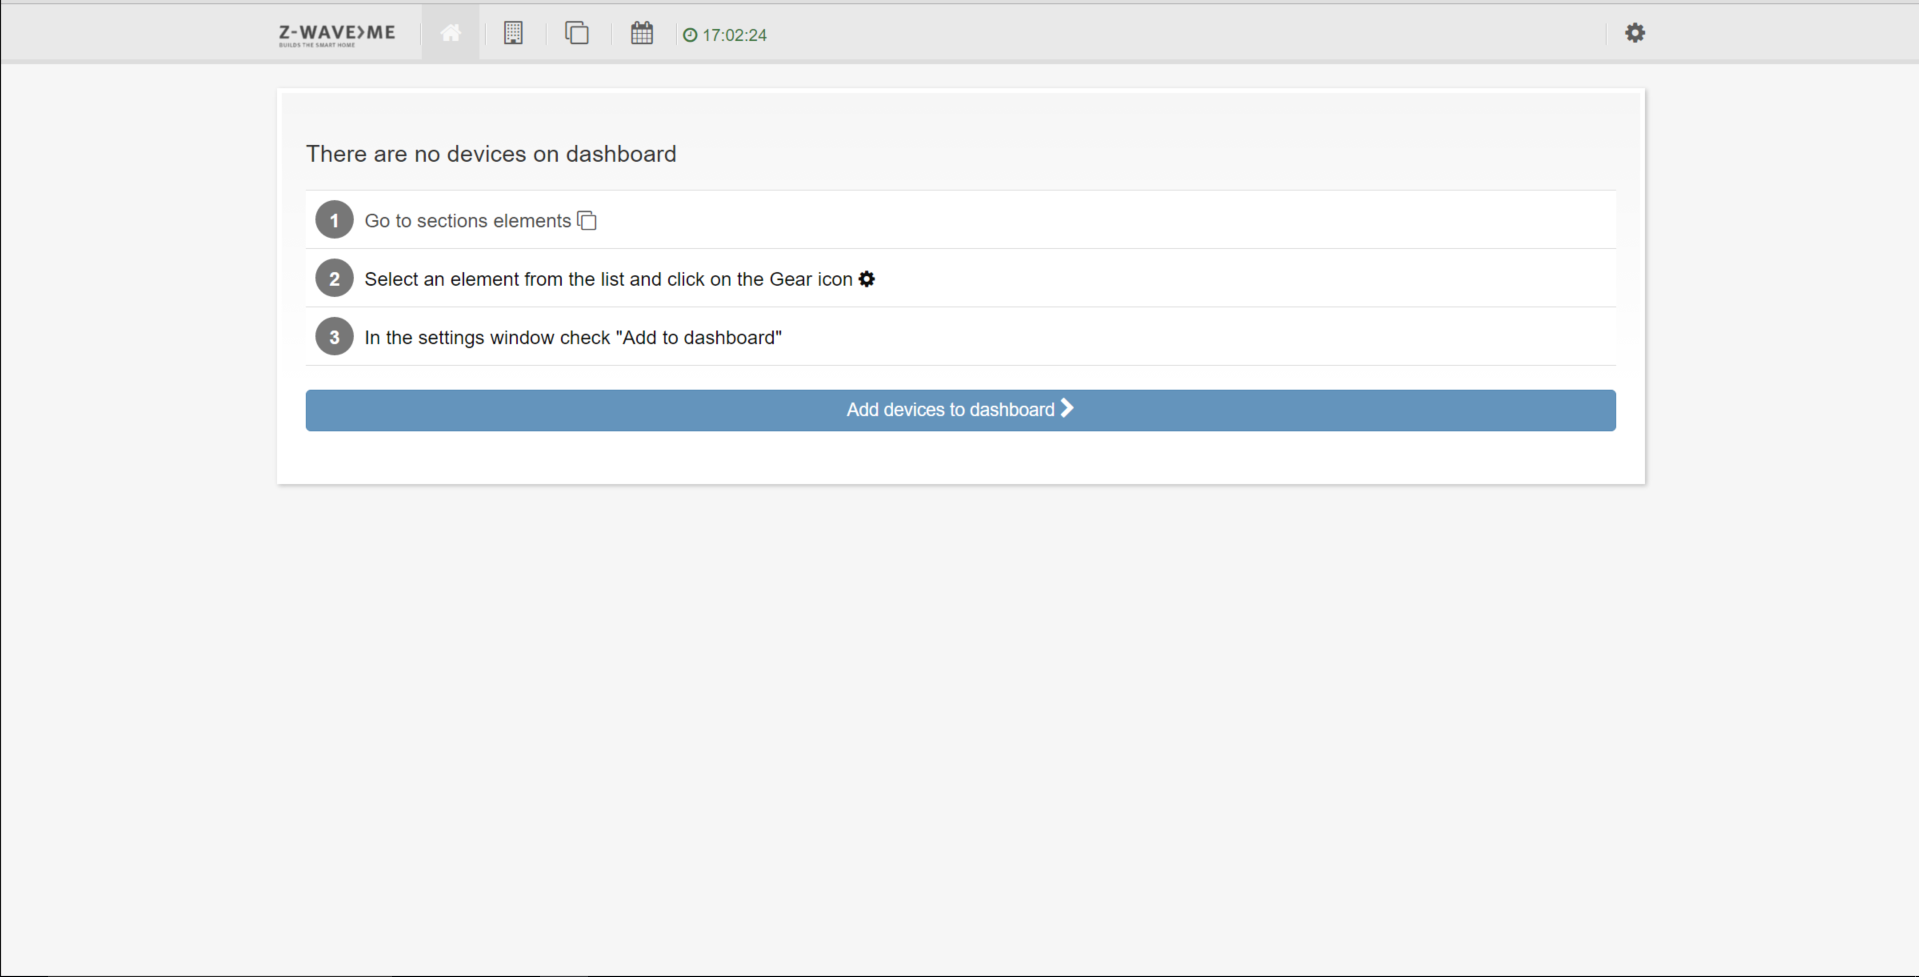
\includegraphics[scale=0.5]{./Images/png/home_zwaveme.png}
	\caption{ZwaveMe menu}
\end{figure}

\item  Pour accéder au mode expert, il faut suivre le lien en haut de l'image

\begin{figure}[h]
	\center
	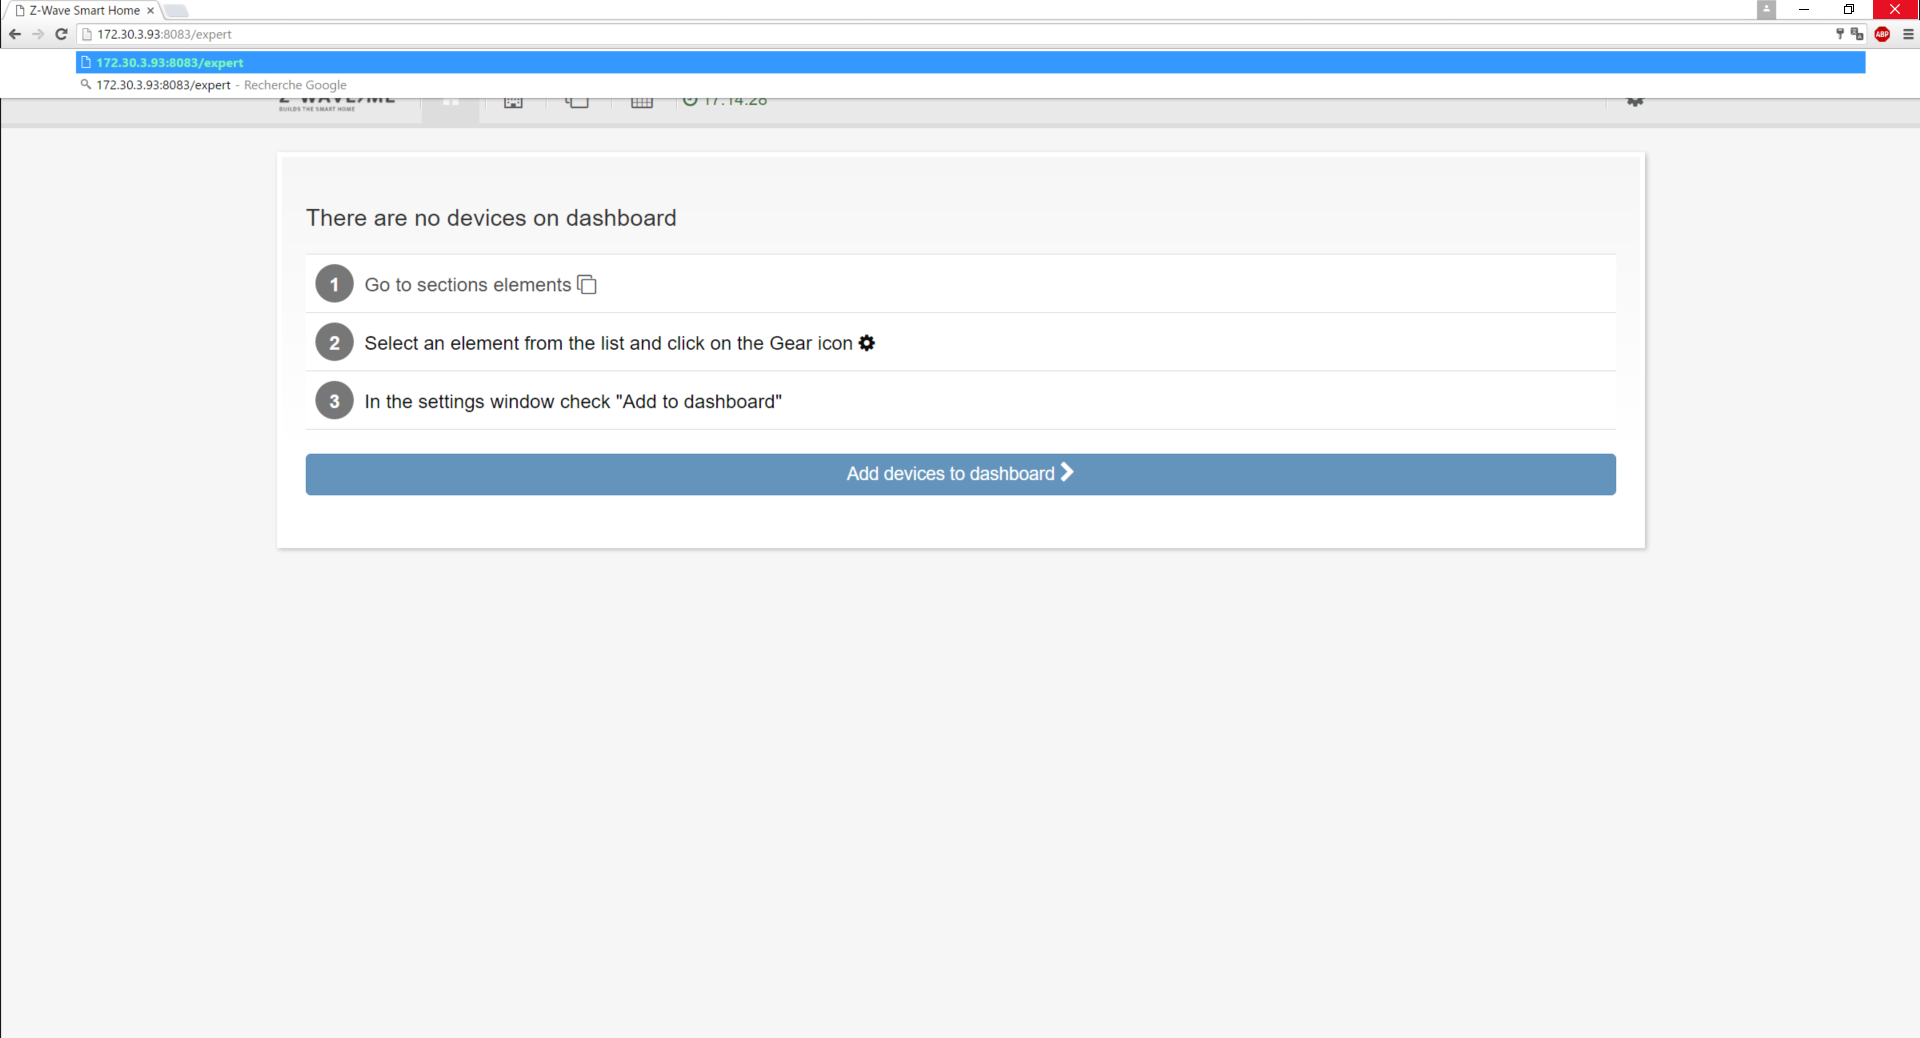
\includegraphics[scale=0.5]{./Images/png/go_to_zwaveme.png}
	\caption{ZwaveMe menu}
\end{figure}

\item Mode expert

\begin{figure}[h]
	\center
	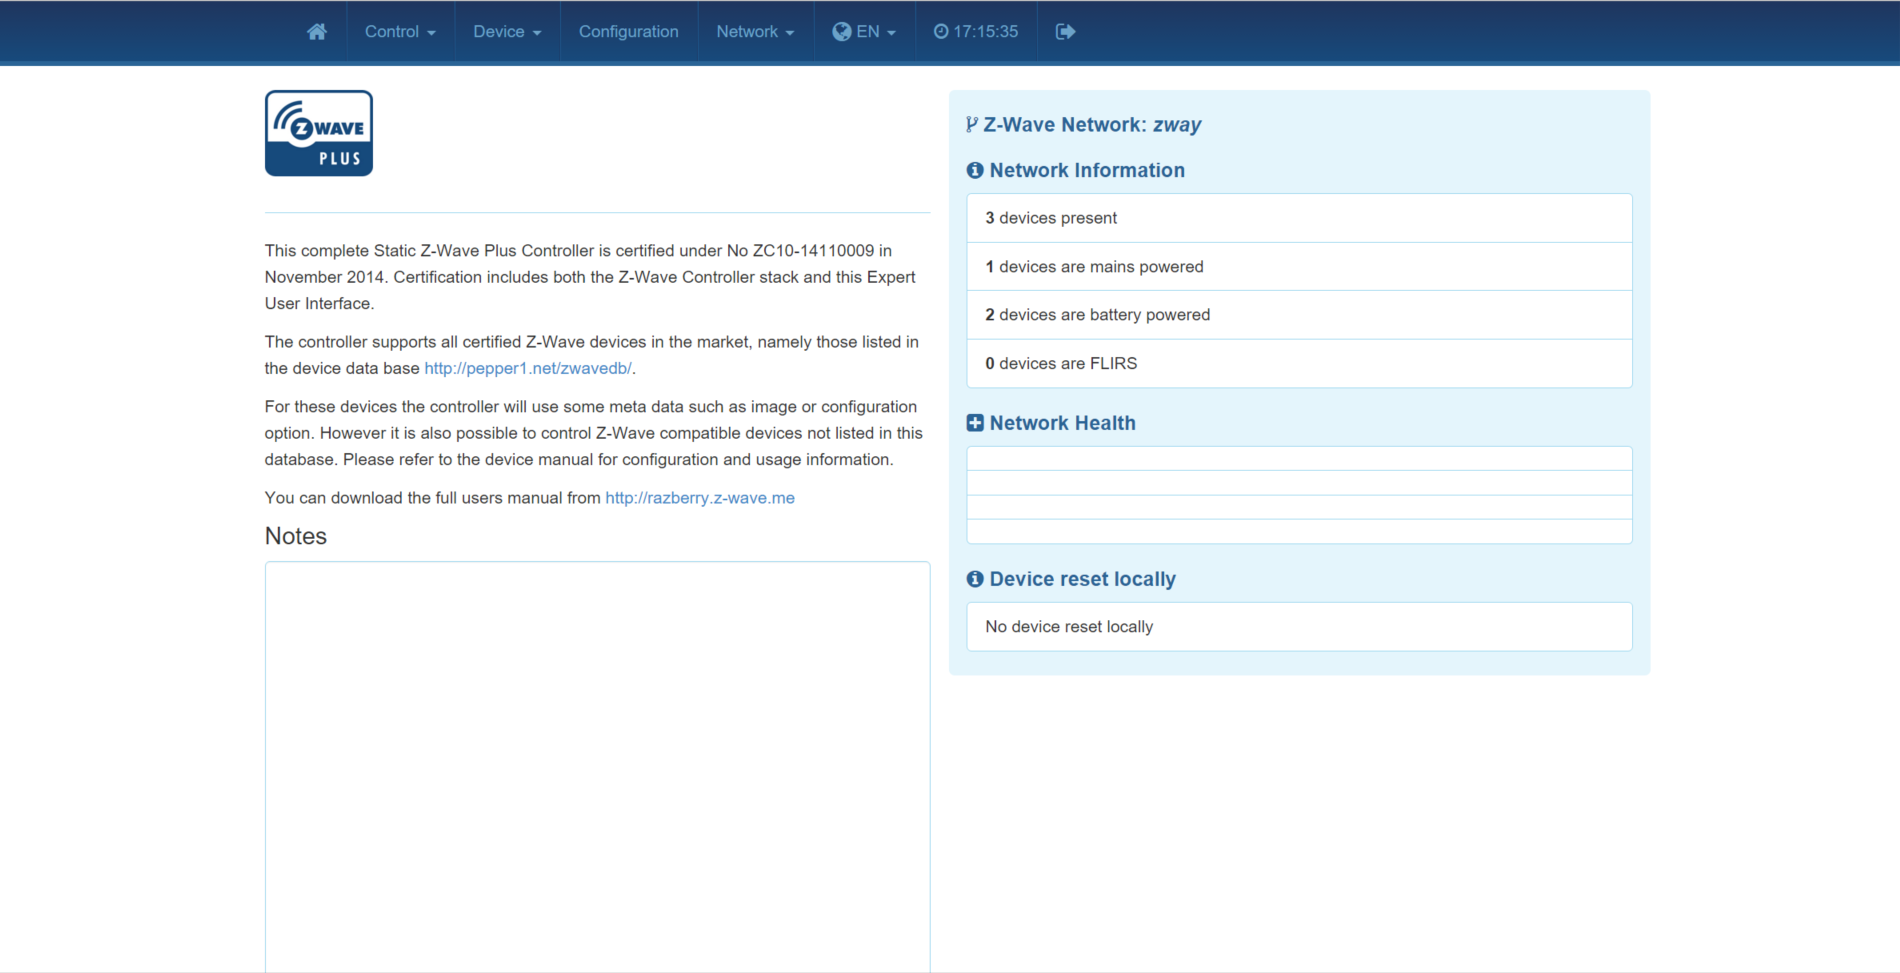
\includegraphics[scale=0.5]{./Images/png/expert_zwaveme.png}
	\caption{ZwaveMe menu expert}
\end{figure}

\subsection{Configuration des capteurs}
Pour gérer vos capteurs, l'interface Web ZWaveMe (mode home) propose une solution.

\begin{figure}[h]
	\center
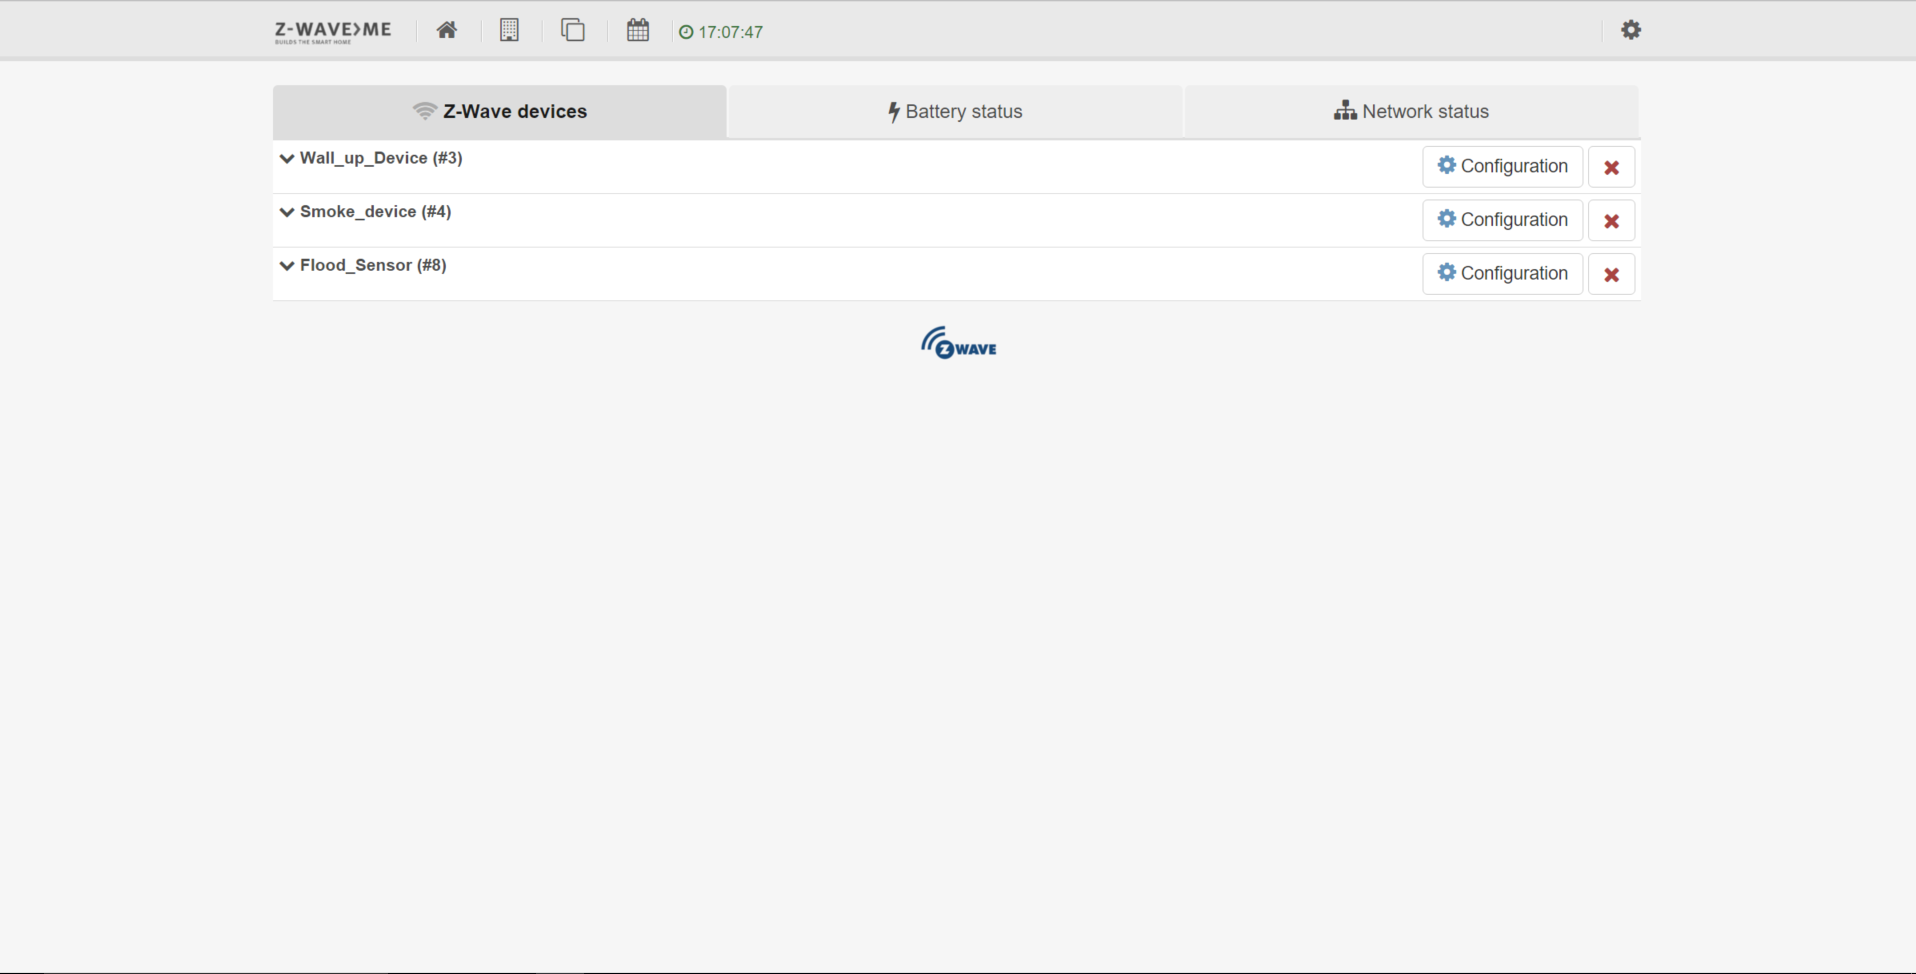
\includegraphics[scale=0.5]{./Images/png/manage_zwaveme.png}
	\caption{ZwaveMe device manager}
\end{figure}

\subsection{Suppression d'un capteur}
Si vous souhaitez supprimer un capteur (un device), vous avez la possibilité en suivant ces images


\item Appuyez sur start exclusion


\begin{figure}[h]
	\center
	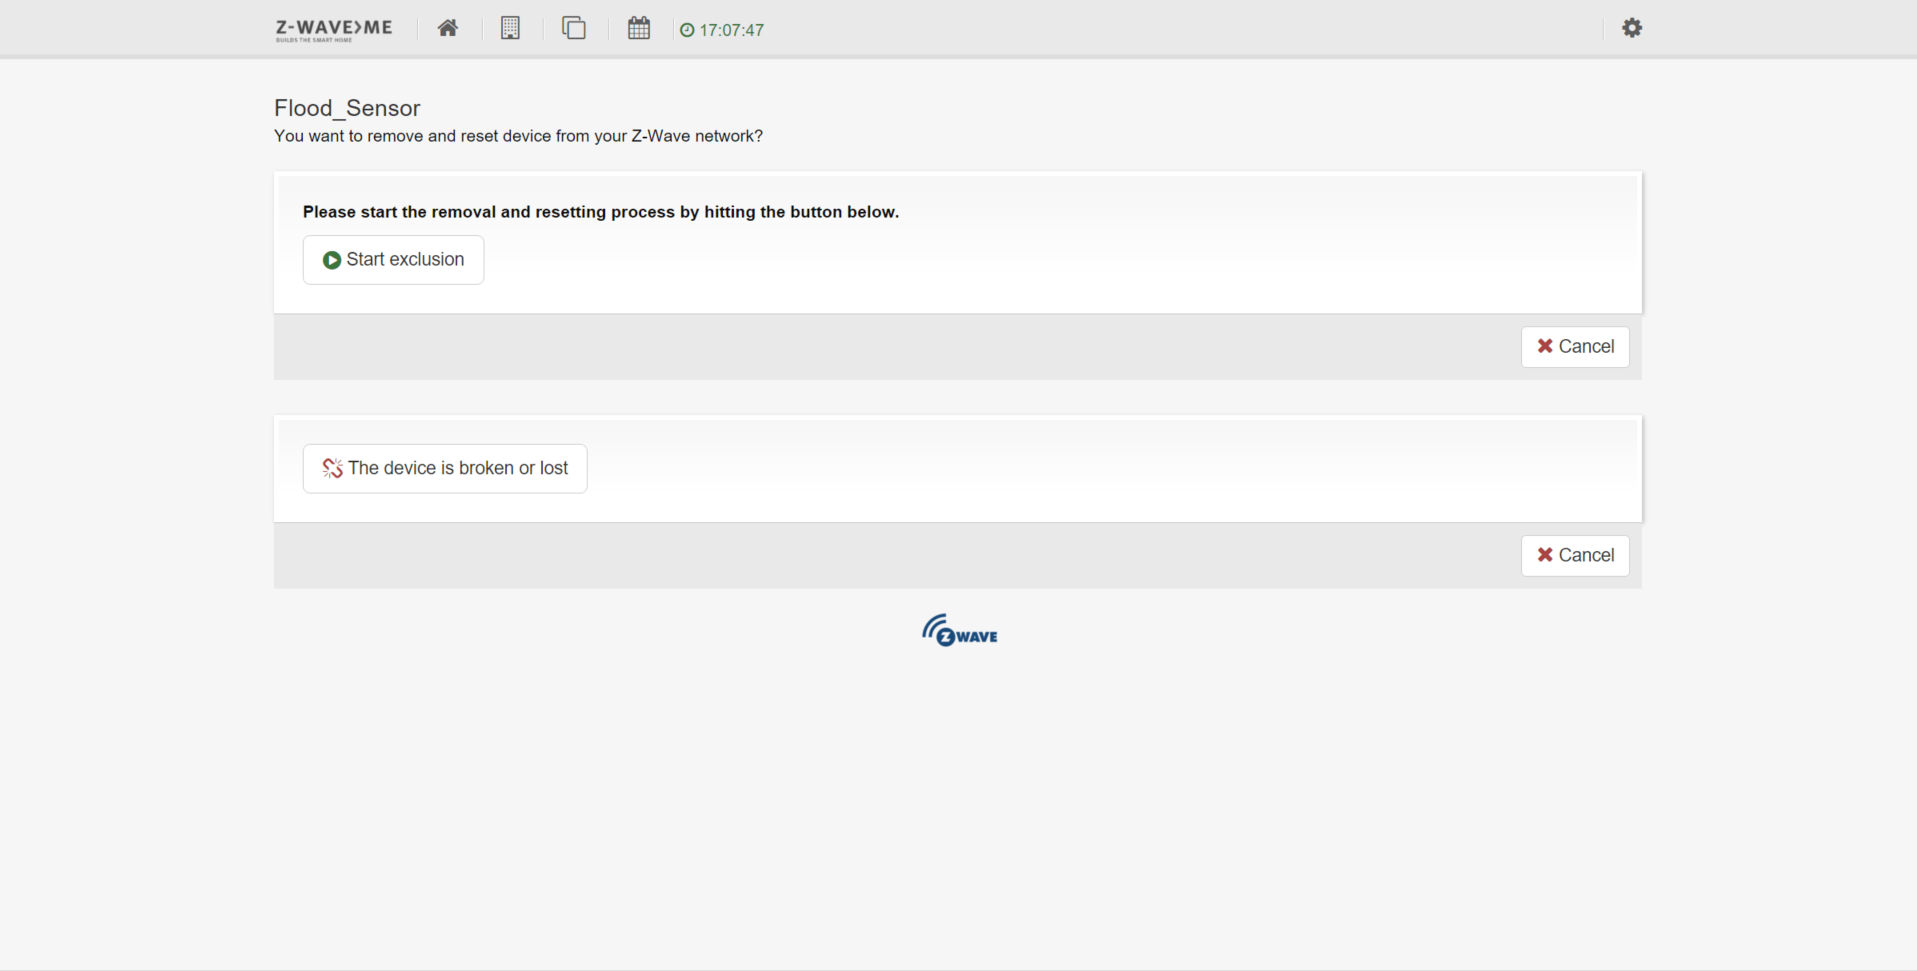
\includegraphics[scale=0.5]{./Images/png/delete_zwaveme.png}
	\caption{ZwaveMe supprimer capteur}
\end{figure}

\begin{figure}[h]
	\center
	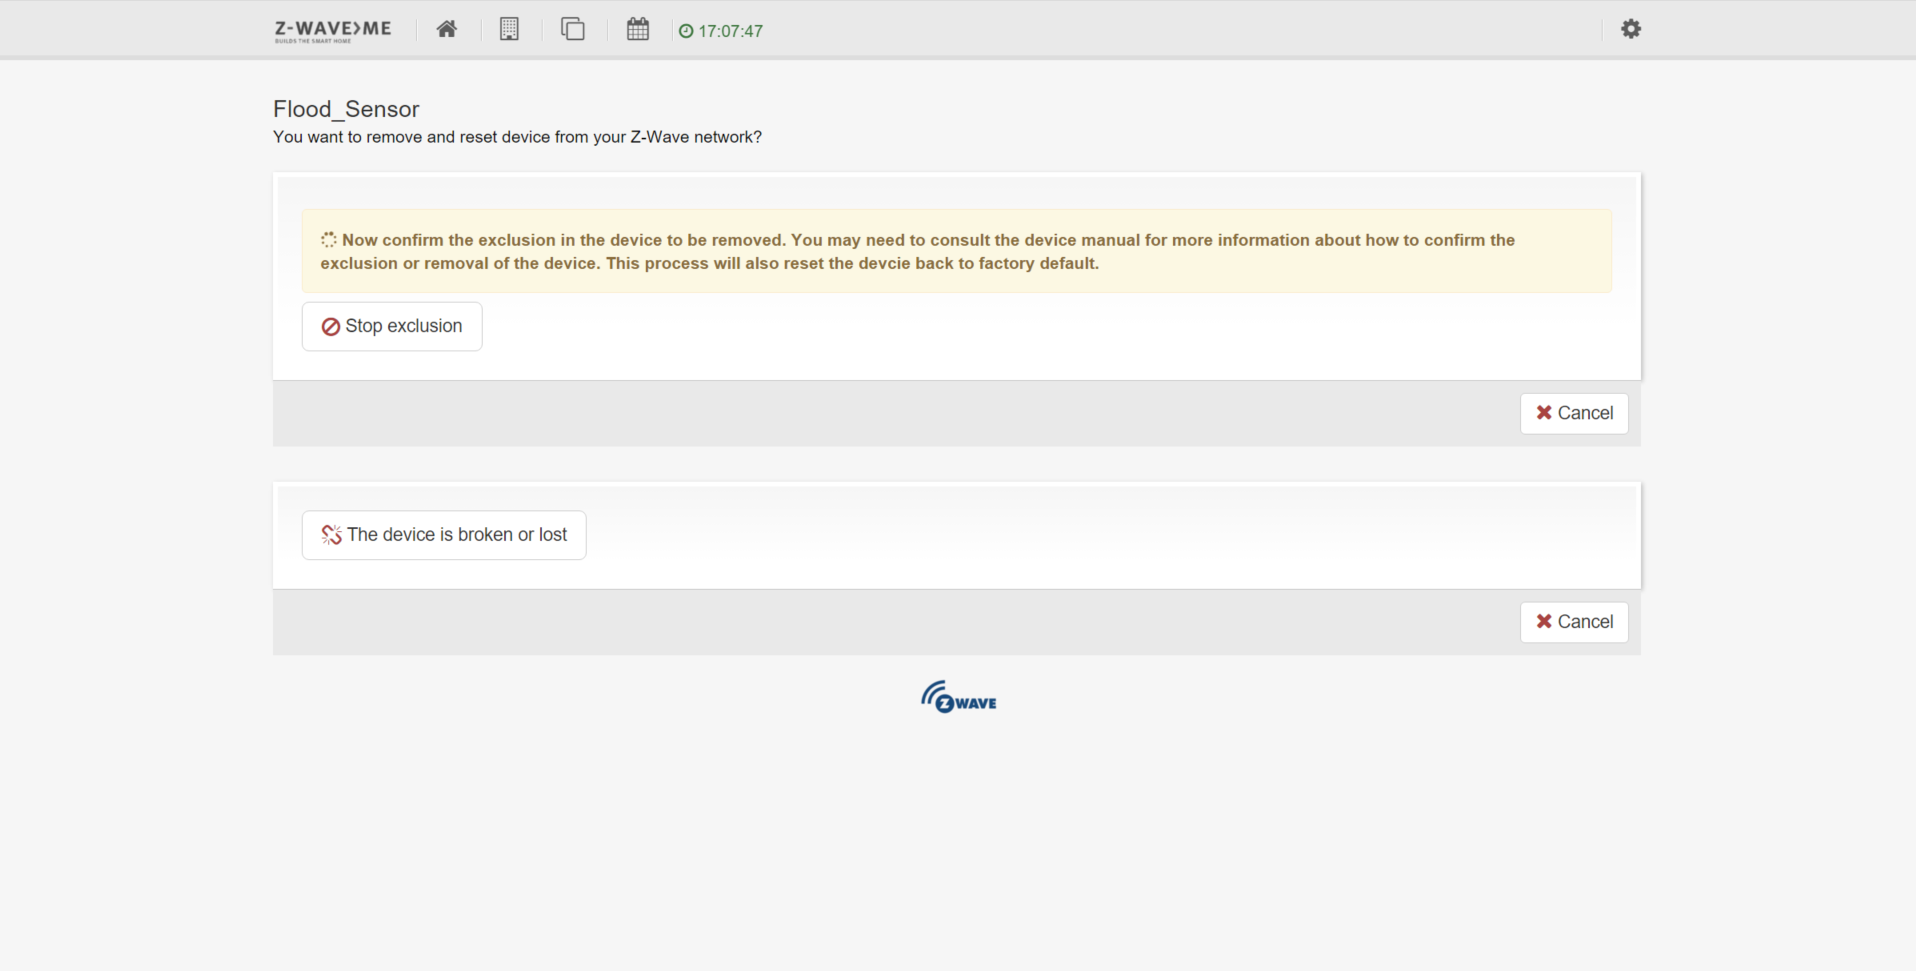
\includegraphics[scale=0.5]{./Images/png/exclusion_zwaveme.png}
	\caption{ZwaveMe exclusion capteur}
\end{figure}

Le device sera alors exclu


\begin{figure}[h]
	\center
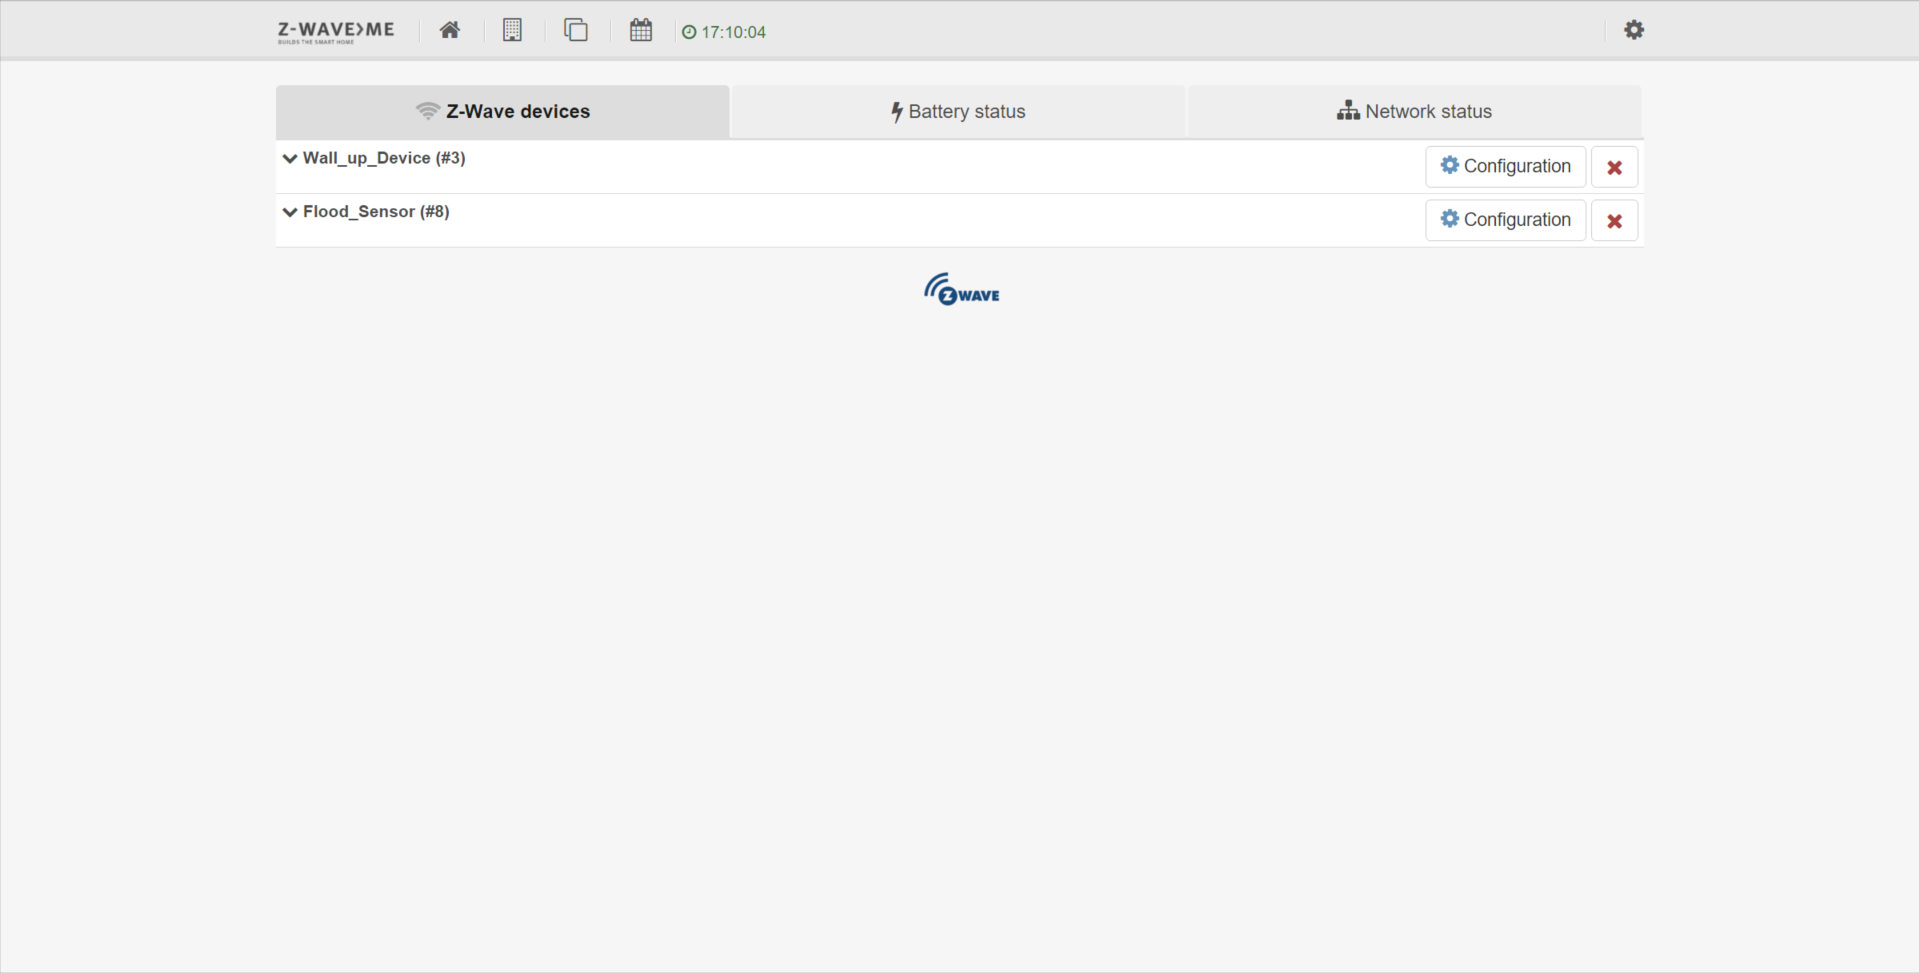
\includegraphics[scale=0.5]{./Images/png/devices_exclu_zwaveme.png}
	\caption{ZwaveMe exclusion capteur}
\end{figure}


\item Les applications disponibles concernant les capteurs.

\begin{figure}[h]
	\center
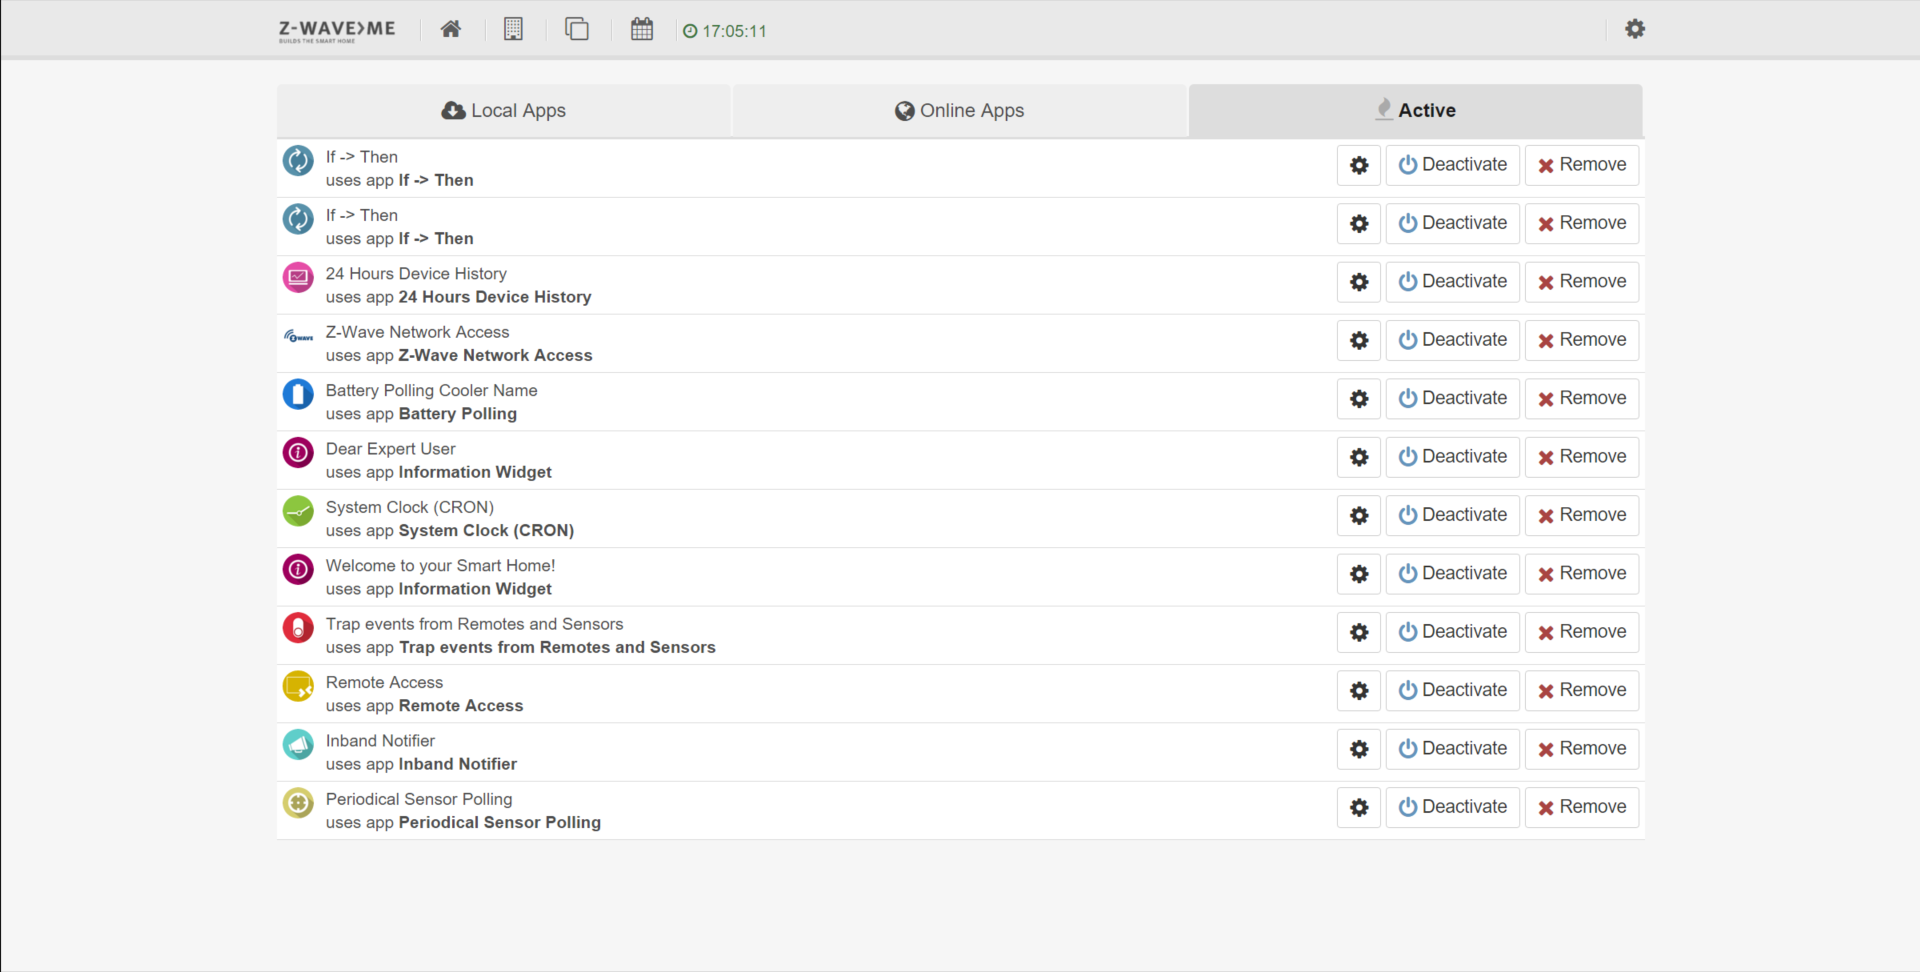
\includegraphics[scale=0.5]{./Images/png/app_zwaveme.png} 
	\caption{Application ZwaveMe}
\end{figure}

\item Dans le mode expert, vous pouvez remarquer l'état de vos capteurs

\begin{figure}[h]
	\center
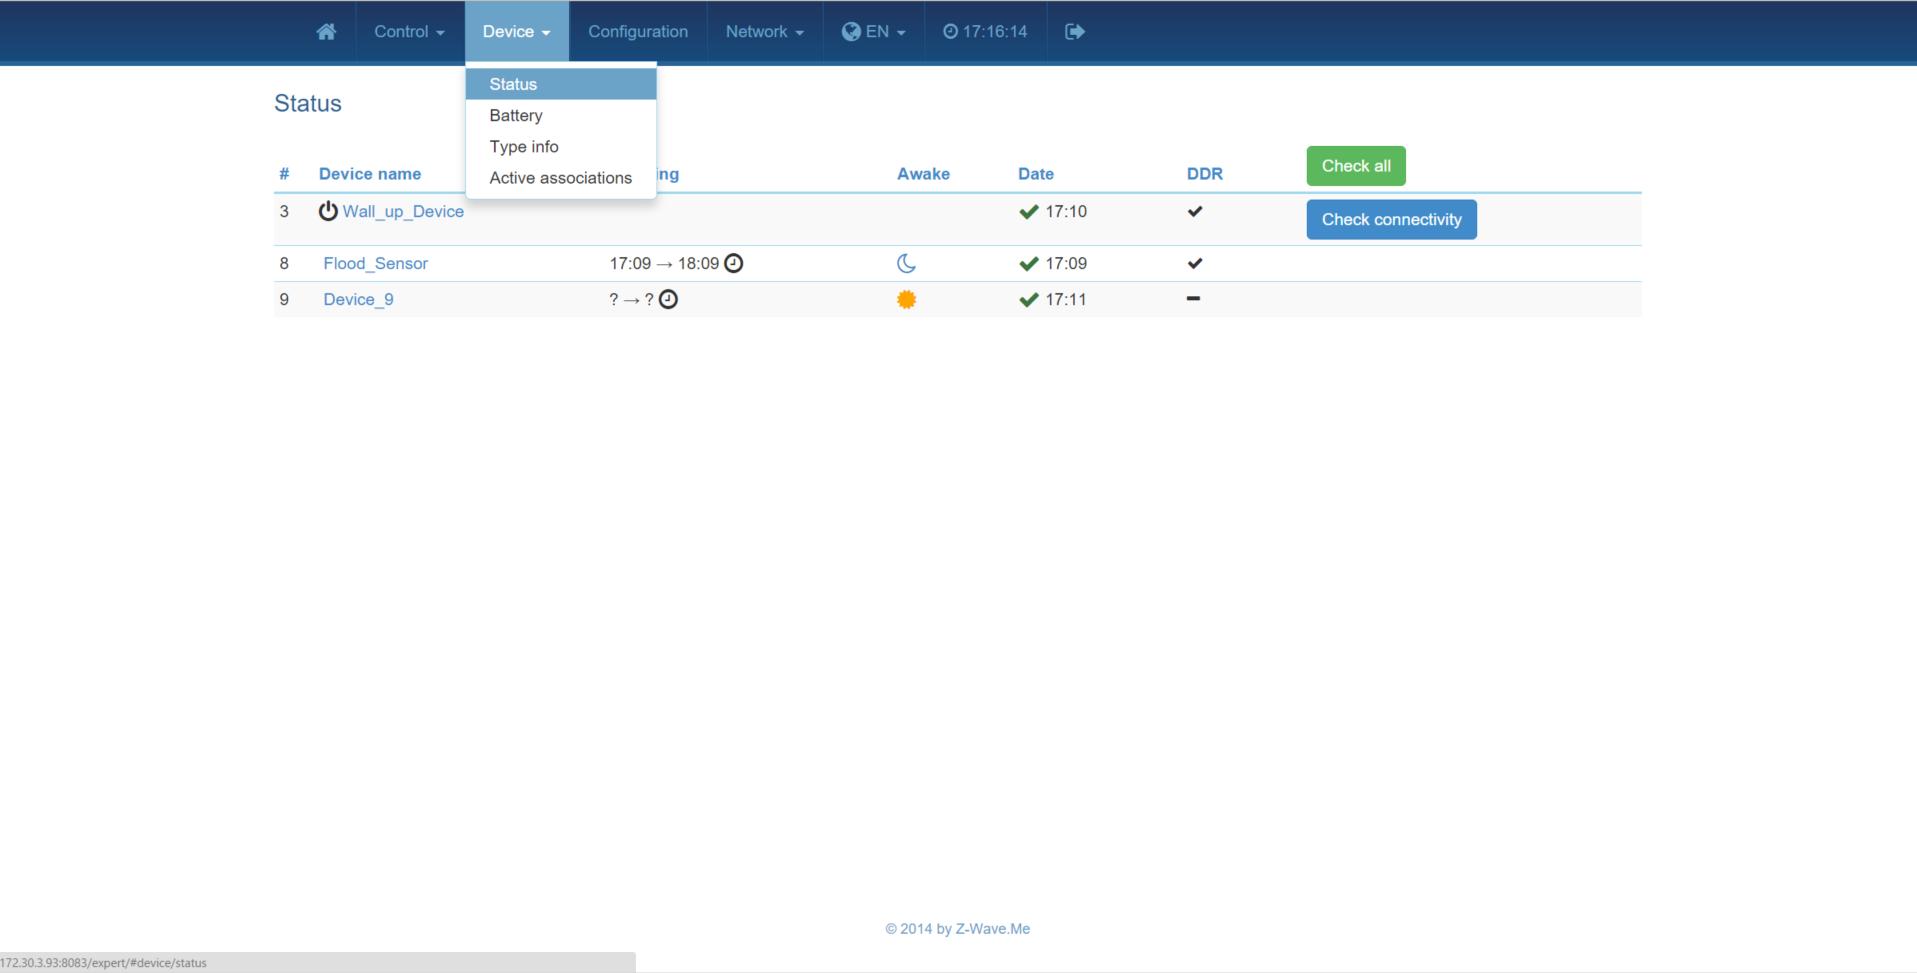
\includegraphics[scale=0.5]{./Images/png/device_Status.png}
	\caption{Status des capteurs ZWaveMe}
\end{figure}


\item Une description détaillée des capteurs disponibles (mode expert)

\begin{figure}[h]
	\center
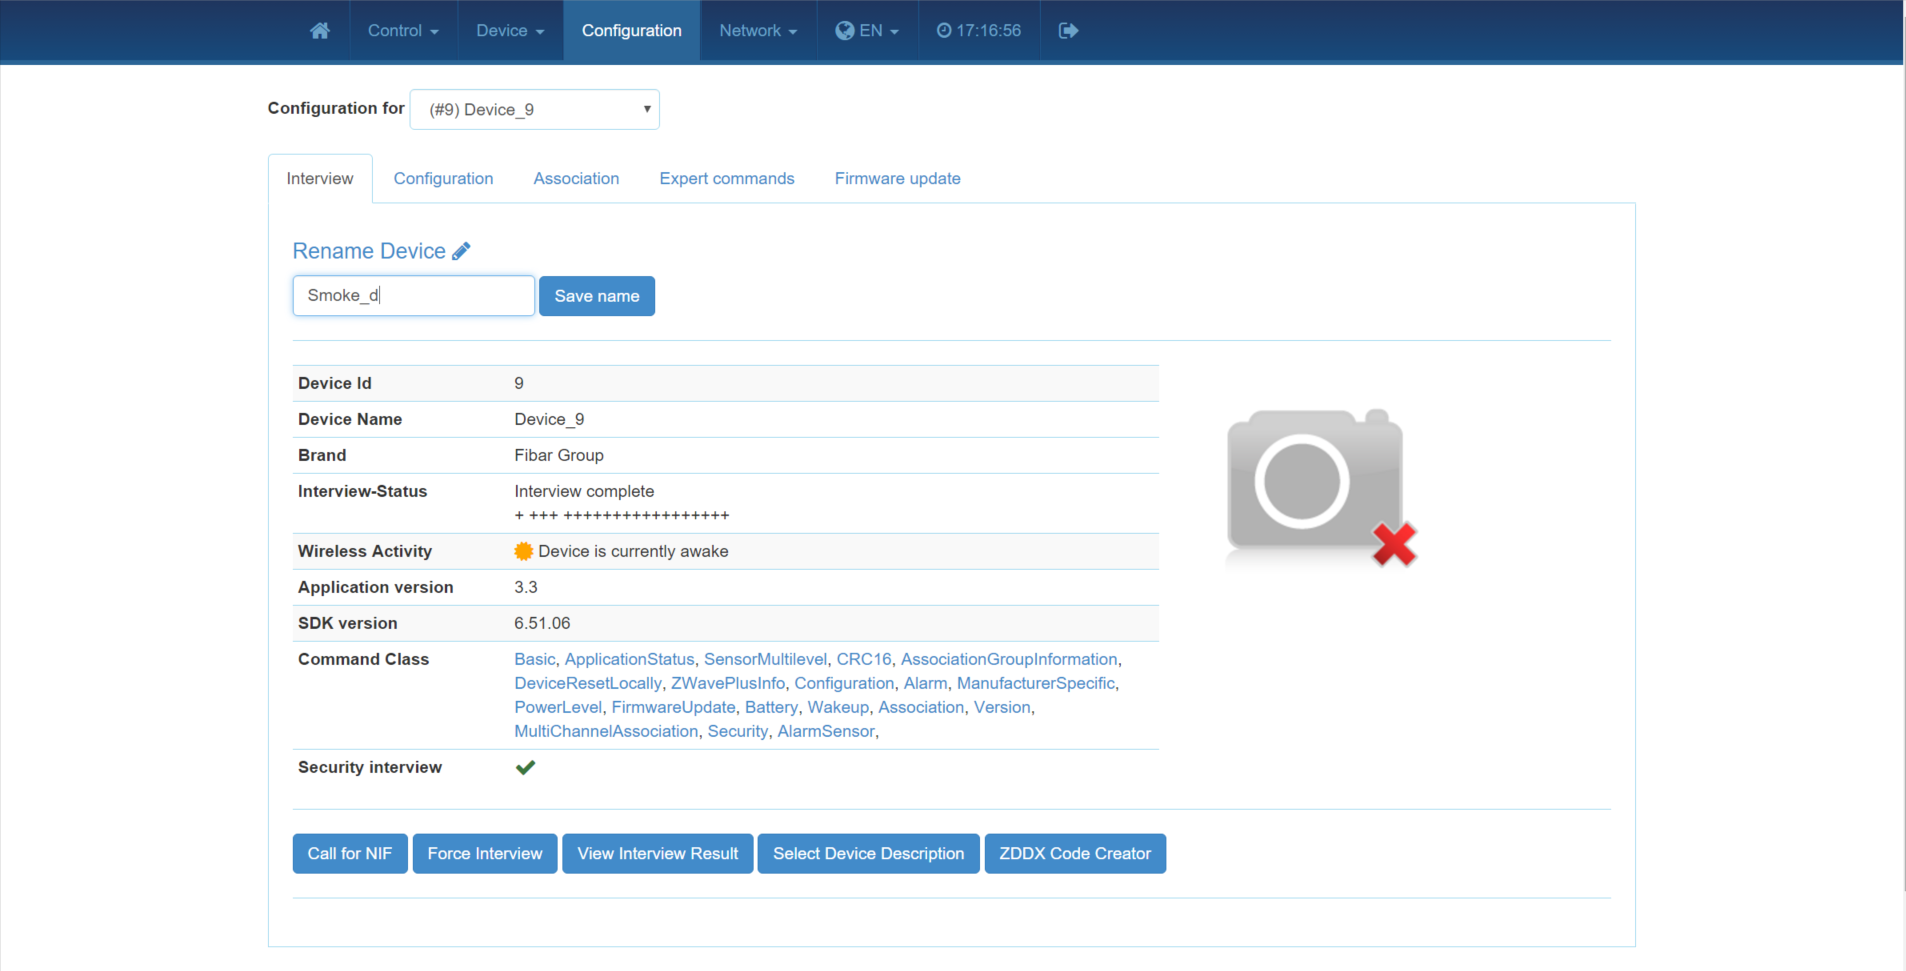
\includegraphics[scale=0.5]{./Images/png/description_zwaveme.png}
	\caption{description device ZWaveMe}
\end{figure}

\item Le log des capteurs qui permet de vérifier l'état des capteurs en temps continu et réel (Veille, On, Off, ...)


\begin{figure}[h]
	\center
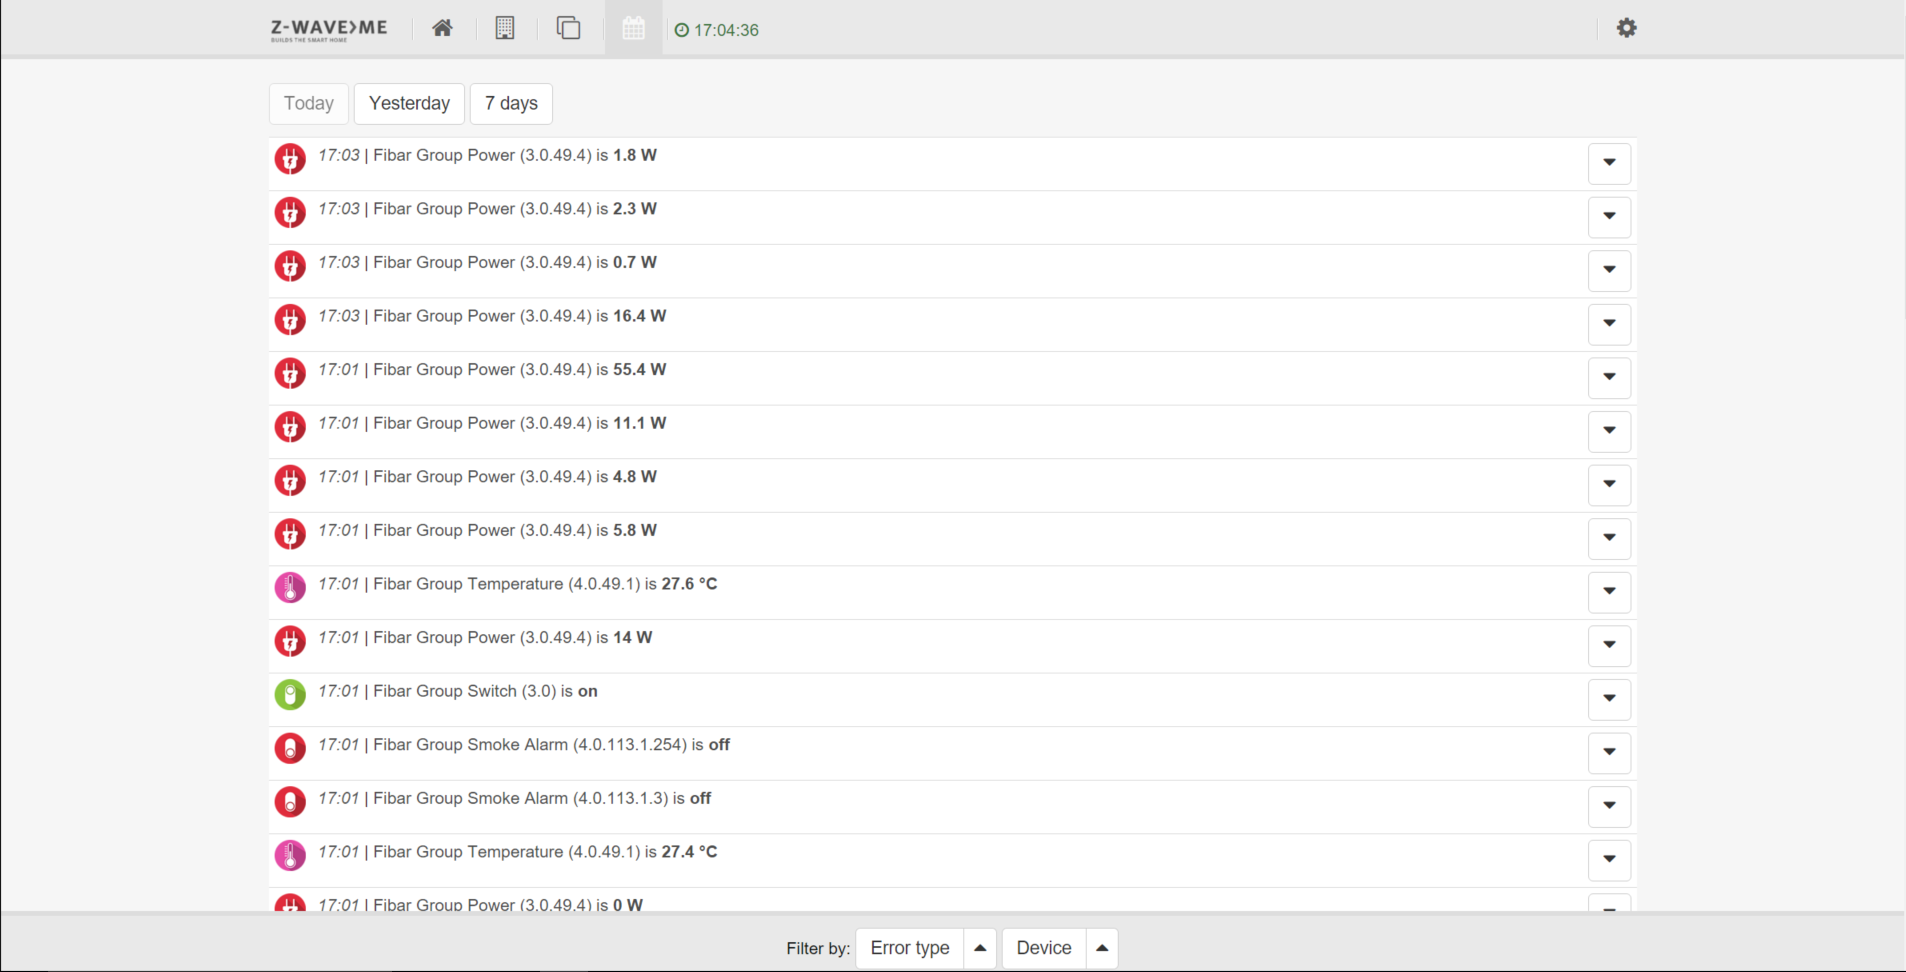
\includegraphics[scale=0.5]{./Images/png/log_zwaveme.png}
	\caption{fichier de journalisation ZWaveMe}
\end{figure}

\item Ajoutez des chambres (Notre application Android se base sur ce principe)

\begin{figure}[h]
	\center
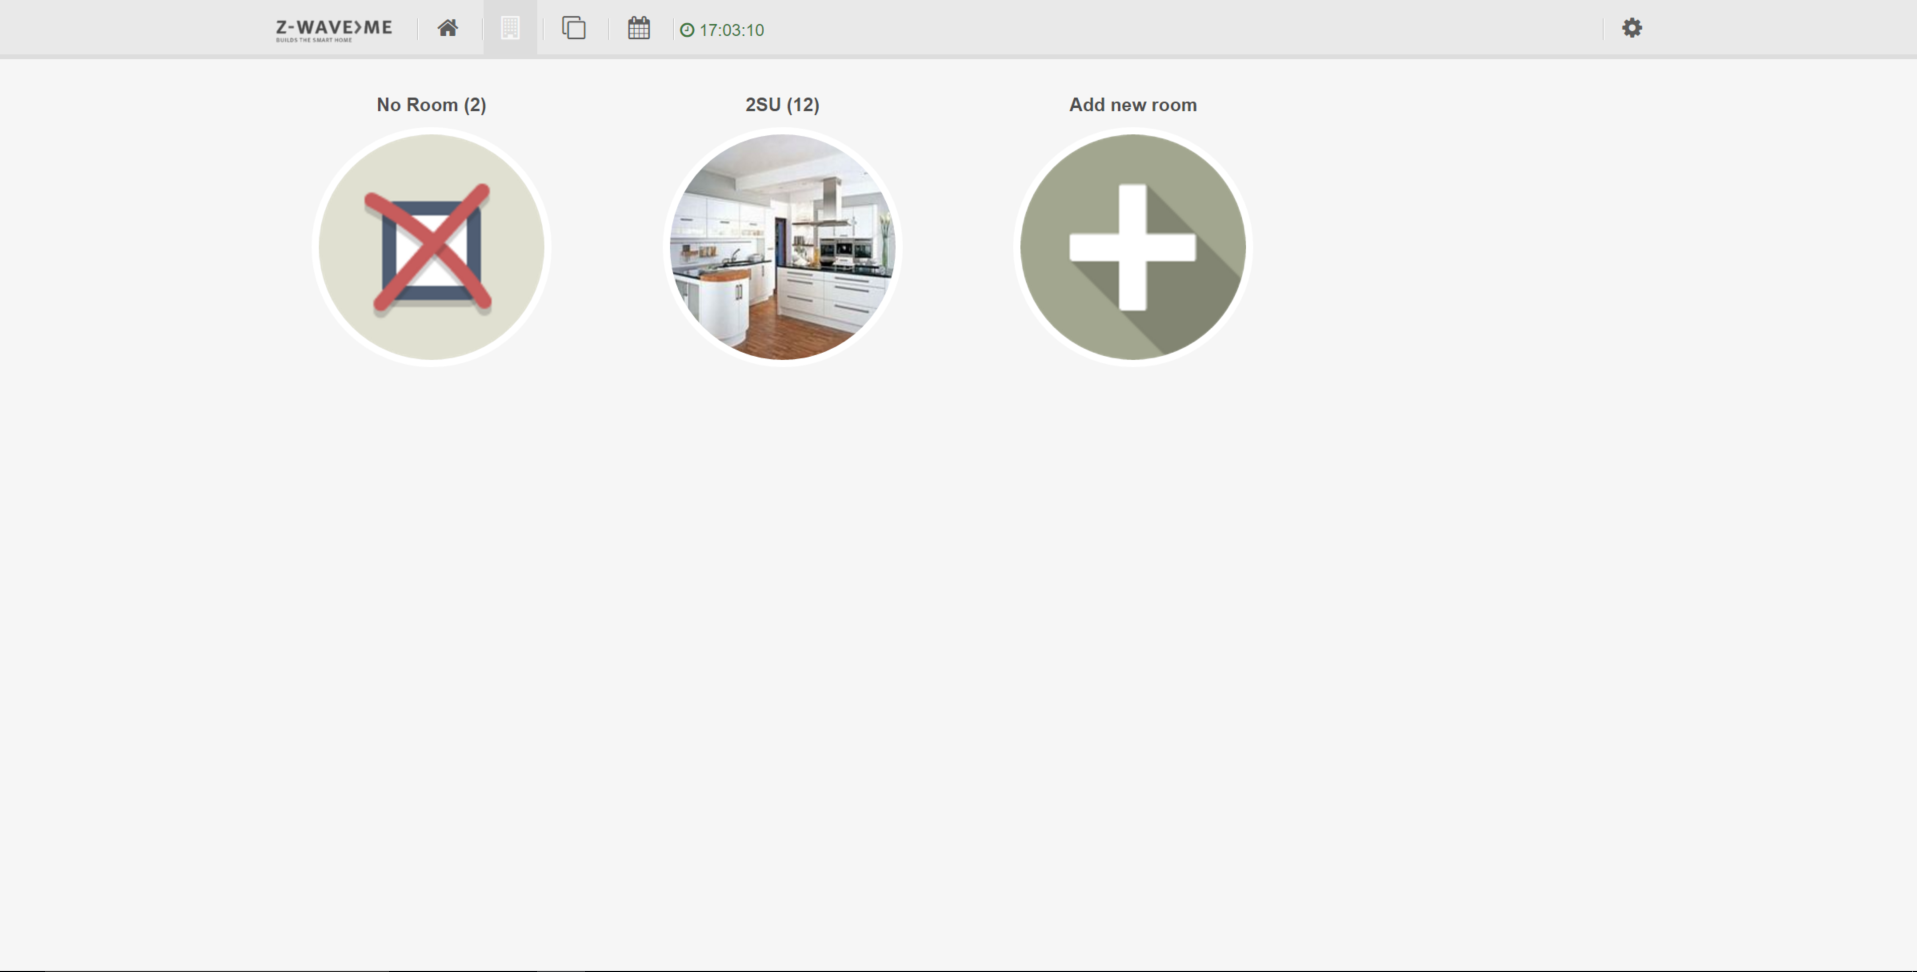
\includegraphics[scale=0.5]{./Images/png/room_zwaveme.png}\newline
%	\caption{pièce dans ZWaveMe}

\item Desciption des capteurs (mode expert)

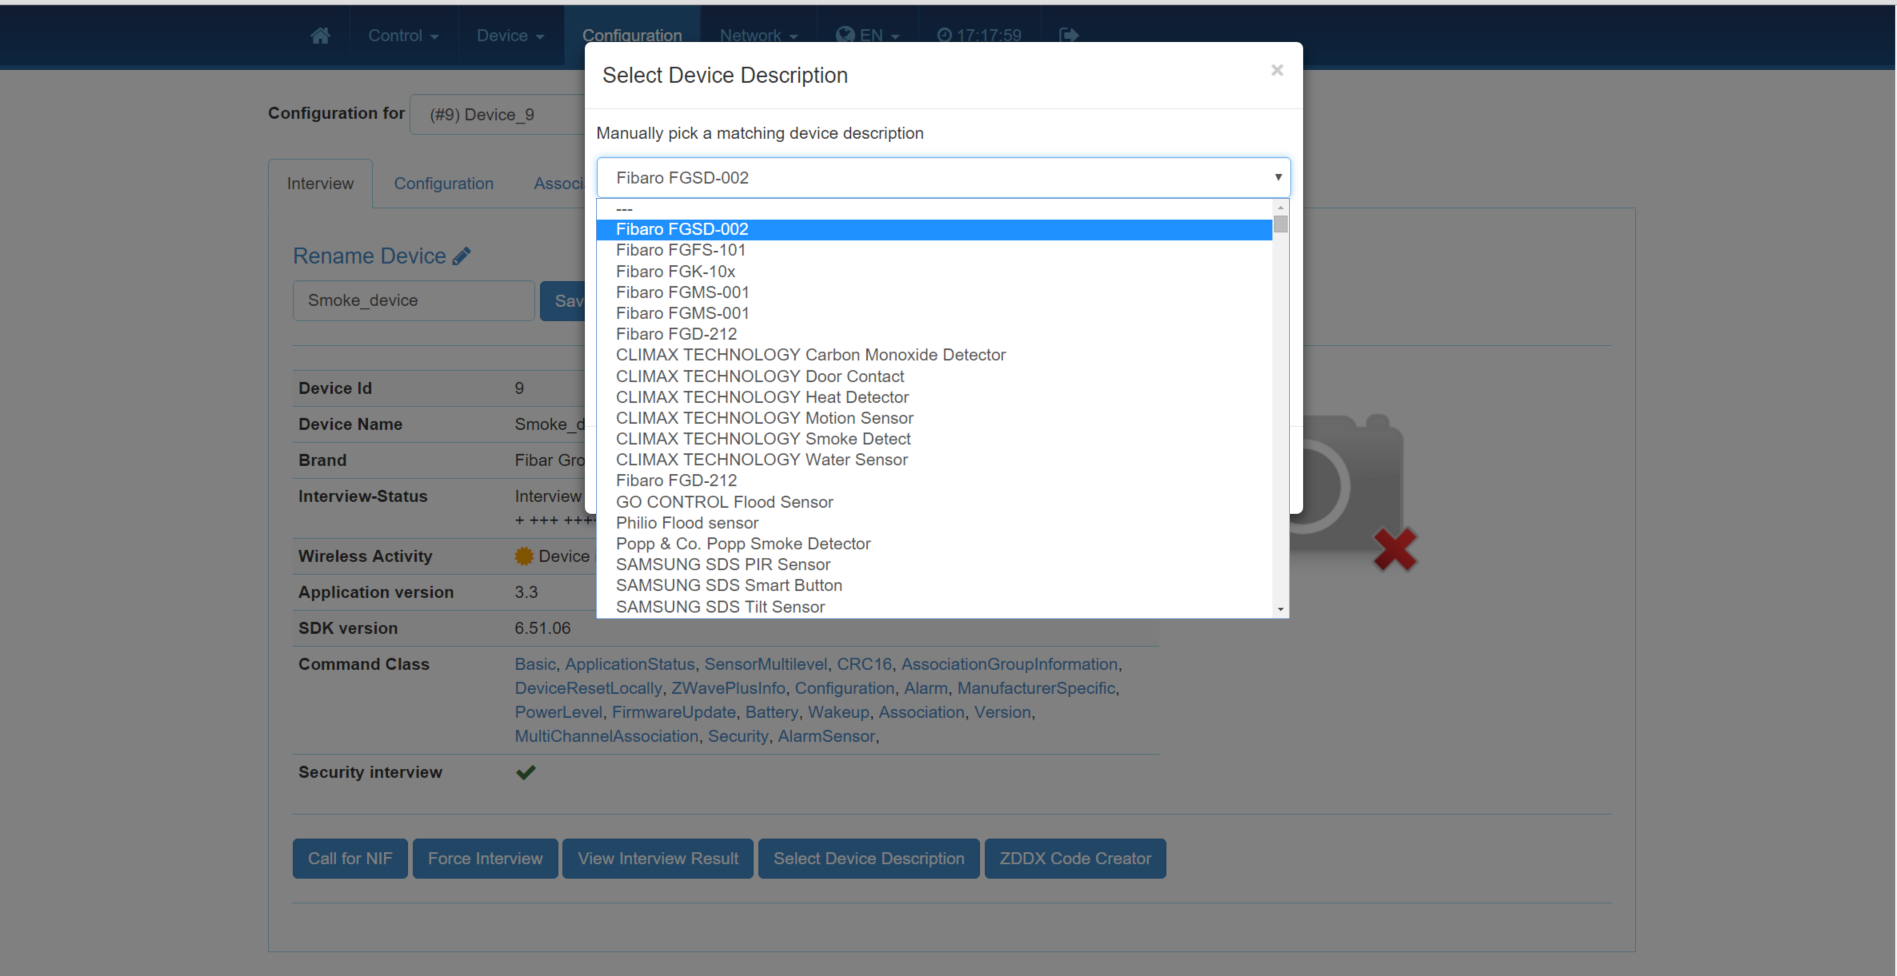
\includegraphics[scale=0.5]{./Images/png/smoke_description_zwaveme.png}
	\caption{Somke\_Sensor description ZWaveMe}
%\end{figure}

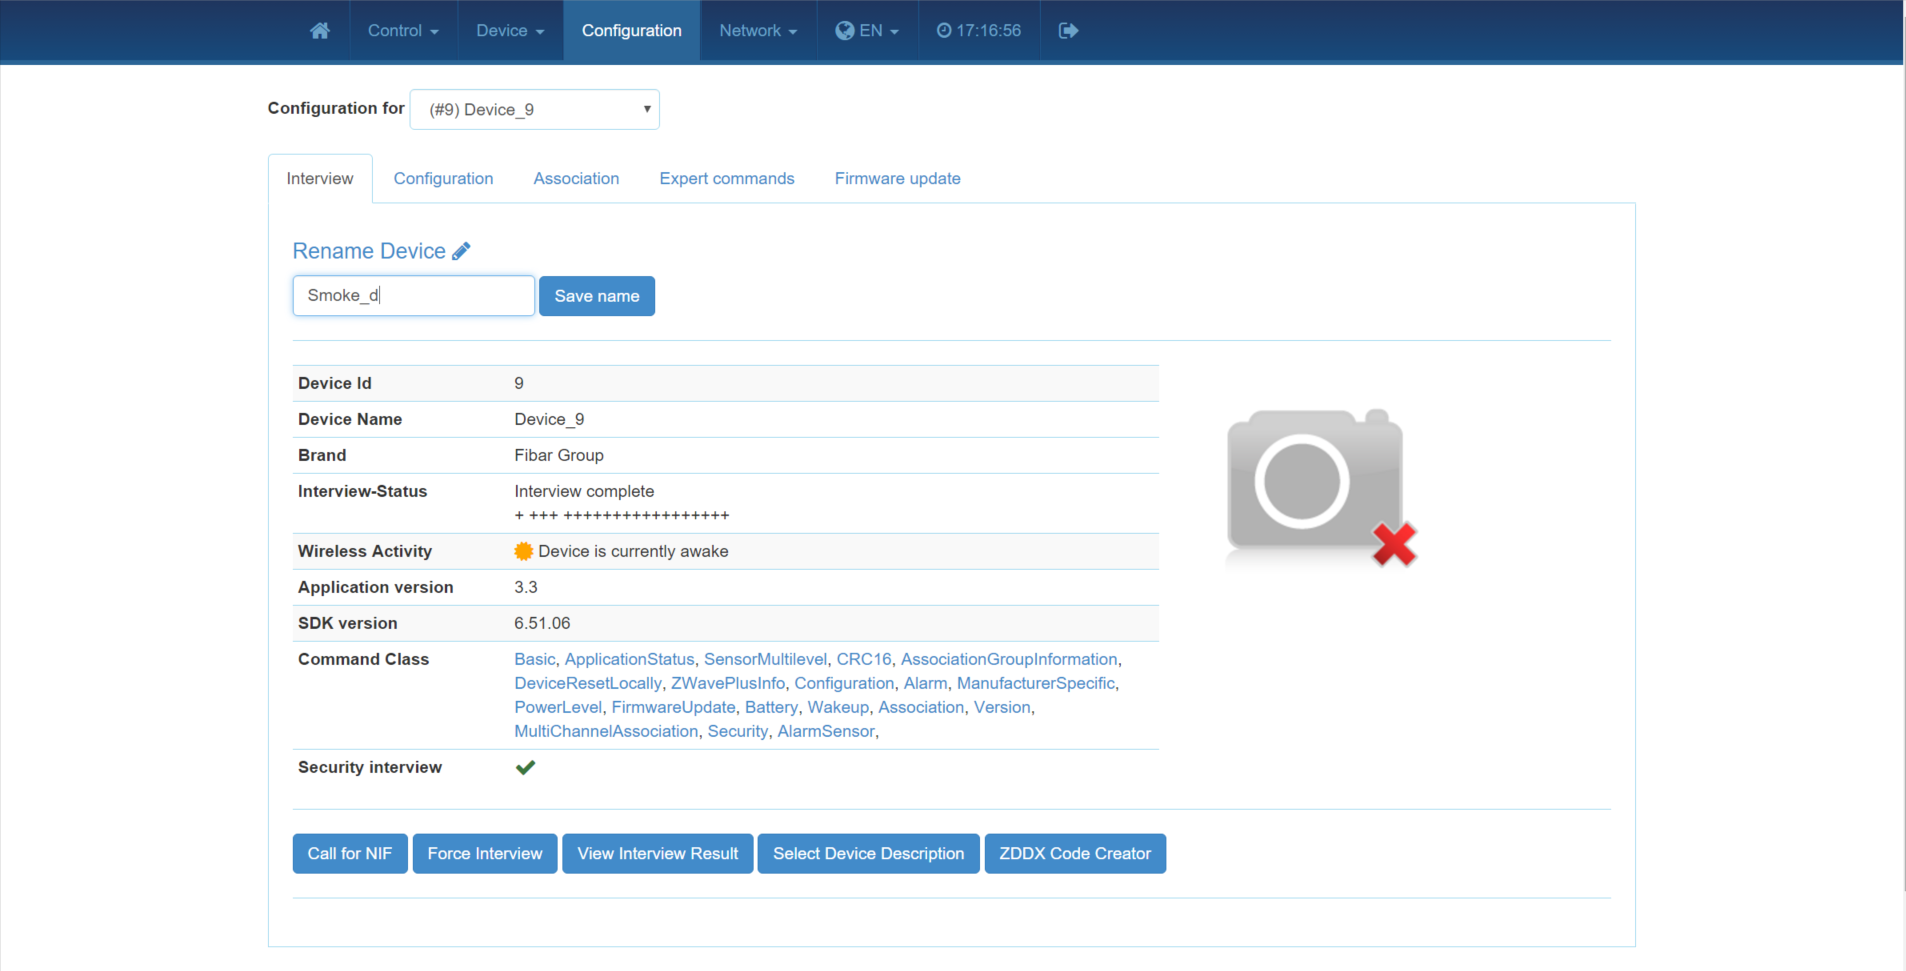
\includegraphics[scale=0.5]{./Images/png/description_zwaveme.png}
%	\caption{description ZWaveMe}

\end{figure}
\end{itemize}


\section{Démonstration}
\begin{itemize}
	\item Une vidéo d'une de nos démonstration sur le flood sensor se trouve sur ce lien
	 \url{https://www.youtube.com/watch?v=nNWe8rKhf1o&feature=youtu.be}
\end{itemize}
\end{document}
